%\section{DATA AND MONTE CARLO SAMPLES}
\chapter{DATA AND MONTE CARLO SAMPLES}
\label{sec:tablessamples}

%Table~\ref{table-data} lists the data samples used in the analysis and their corresponding luminosities.
%The signal samples and their cross-section times branchig-ratio values are reported in Table~\ref{table-mcsignal}.
%Table~\ref{table-bkg} provides the background datasets, along with their cross sections and luminosities.

\begin{table}
\caption{Data samples used in the analysis.}
\label{table-data}
\vspace{\medskipamount}
\begin{center}
\footnotesize
\begin{tabular}{|l|l|r|}
\hline
Channel & Dataset & Luminosity [pb$^{-1}$] \\
\hline
$2\mu2q$ & /DoubleMu/Run2012A-13Jul2012-v1/AOD & 808\\
         & /DoubleMu/Run2012A-recover-06Aug2012-v1/AOD & 82\\
         & /DoubleMu/Run2012B-13Jul2012-v4/AOD & 4429 \\
         & /DoubleMu/Run2012C-24Aug2012-v1/AOD & 495 \\
         & /DoubleMu/Run2012C-EcalRecover\_11Dec2012-v1/AOD & 134\\
         & /DoubleMu/Run2012C-PromptReco-v2/AOD & 6394\\
         & /DoubleMu/Run2012D-PromptReco-v1/AOD & 7274\\
\hline 
$2e2q$   & /DoubleElectron/Run2012A-13Jul2012-v1/AOD & 808\\
         & /DoubleElectron/Run2012A-recover-06Aug2012-v1/AOD & 82\\
         & /DoubleElectron/Run2012B-13Jul2012-v4/AOD & 4429\\
         & /DoubleElectron/Run2012C-24Aug2012-v1/AOD & 495\\
         & /DoubleElectron/Run2012C-EcalRecover\_11Dec2012-v1/AOD & 134\\
         & /DoubleElectron/Run2012C-PromptReco-v2/AOD & 6394\\
         & /DoubleElectron/Run2012D-PromptReco-v1/AOD & 7274\\
\hline 
$e\mu qq$& /MuEG/Run2012A-13Jul2012-v1/AOD & 808\\
         & /MuEG/Run2012A-recover-06Aug2012-v1/AOD & 82\\
         & /MuEG/Run2012B-13Jul2012-v4/AOD & 4429\\
         & /MuEG/Run2012C-24Aug2012-v1/AOD & 495\\
         & /MuEG/Run2012C-EcalRecover\_11Dec2012-v1/AOD & 134\\
         & /MuEG/Run2012C-PromptReco-v2/AOD & 6394\\
         & /MuEG/Run2012D-PromptReco-v1/AOD & 7274\\
\hline
\end{tabular}
\end{center}
\end{table}

%\begin{table}[htpb]
\begin{table}
\caption{ 
The signal samples, $\Htollqq$ ($\ell = \mathrm{e}, \mu, \tau$),
simulated with POWHEG are
\textit{/GluGluToHToZZTo2L2Q\_M-xyz\_8TeV-powheg-pythia6/Summer12\_DR53X-PU\_S10\_START53\_V7A-v1/AODSIM}, where $xyz$ is the Higgs boson mass hypothesis, $\MH$. The cross section times branching fraction for each $m_H$ value is listed in pb. Each sample was generated with 300,000 events.}
\label{table-mcsignal}
\vspace*{\medskipamount}
\begin{center}
\small
\begin{tabular}{|c|c|}
\hline
$\MH$ ($\GeVcc$) & $\sigma\times$ Br($\Htollqq$) [pb] \\ \hline
200  &  0.2566 \\ % \hline
 210  &  0.2538  \\ % \hline
 220  &  0.2416  \\ % \hline
 230  &  0.2278  \\ % \hline
 250  &  0.2022 \\ % \hline
 275  &  0.1751  \\ % \hline
 300  &  0.1563  \\ % \hline
 325  &  0.1478  \\ % \hline
 350  &  0.1482  \\         
 375  &  0.1360  \\       
 400  &  0.1111 \\ % \hline
 425  &  0.0914 \\ % \hline
 450  &  0.7311 \\ % \hline
 475  &  0.6000 \\ % \hline
 500  &  0.4719 \\ % \hline
  525  &  0.0380 \\ % \hline
  550  &  0.0305 \\ % \hline
 575  &  0.0250 \\ % \hline
  600  &  0.0201 \\ \hline 
 
\end{tabular}
\end{center}
\end{table}

\begin{table}[htpb]
\caption{ 
Background simulated samples of the Summer12 production used in the analysis.
The equivalent luminosity of the processed events for each sample is 
computed using the (N)NLO cross section in the $3^\mathrm{rd}$ column.
}
\label{table-bkg}
\vspace*{\medskipamount}
\begin{center}
\footnotesize
\begin{tabular}{|l|l|c|c|}
\hline
Process & dataset & $\sigma$ [pb]& luminosity [$\invfb$] \\
\hline 
 & & & \\
$Z$+jets       & /DYJetsToLL\_M-50\_TuneZ2Star\_8TeV-madgraph-tarball/ & 3503.71 & 8.7 \\
(inclusive)    & Summer12\_DR53X-PU\_S10\_START53\_V7A-v1/AODSIM & & \\
 & & & \\
$Z$+1 jet      & /DY1JetsToLL\_M-50\_TuneZ2Star\_8TeV-madgraph/ & 660.6 & 36.4\\
(exclusive)    & Summer12\_DR53X-PU\_S10\_START53\_V7A-v1/AODSIM  & & \\
$Z$+2 jet      & /DY2JetsToLL\_M-50\_TuneZ2Star\_8TeV-madgraph/ & 215.1 & 101.6 \\
(exclusive)    & Summer12\_DR53X-PU\_S10\_START53\_V7A-v1/AODSIM  & & \\
$Z$+3 jet      & /DY3JetsToLL\_M-50\_TuneZ2Star\_8TeV-madgraph/ & 65.79 & 167.4 \\
(exclusive)    & Summer12\_DR53X-PU\_S10\_START53\_V7A-v1/AODSIM  & & \\
$Z$+4 jet      & /DY4JetsToLL\_M-50\_TuneZ2Star\_8TeV-madgraph/ & 27.59 & 232.1 \\
(exclusive)    & Summer12\_DR53X-PU\_S10\_START53\_V7A-v1/AODSIM  & & \\
 & & & \\
$\Pqt \Paqt$ & /TTTo2L2Nu2B\_8TeV-powheg-pythia6/ & 23.38 & 461 \\
         & Summer12\_DR53X-PU\_S10\_START53\_V7A-v1/AODSIM  & & \\
$ZZ$ & /ZZ\_TuneZ2star\_8TeV\_pythia6\_tauola/ & 17.654 & 549 \\
     & Summer12\_DR53X-PU\_S10\_START53\_V7A-v1/AODSIM  & & \\
$WZ$ & /WZ\_TuneZ2star\_8TeV\_pythia6\_tauola/ & 22.88 & 424 \\
     & Summer12\_DR53X-PU\_S10\_START53\_V7A-v1/AODSIM  & & \\
$WW$ & /WW\_TuneZ2star\_8TeV\_pythia6\_tauola/ & 57.1097 & 168 \\
     & Summer12\_DR53X-PU\_S10\_START53\_V7A-v1/AODSIM  & & \\
 & & & \\
\hline
\end{tabular}
\end{center}
\end{table}


\chapter{TRIGGER EFFICIENCIES AND MONTE CARLO CORRECTION FACTORS}
\label{sec:hltsf}
The trigger efficiencies and MC correction factors used in the analysis are listed in Tables~\ref{elleg8SF} and~\ref{elleg17SF} for the electron
triggers, and in Table~\ref{dimuoneff} for the muon trigger.

\begin{table}[h]
\caption{Working point loose to the HLT Ele8 leg tag-and-probe efficiencies and scale factors.}
\label{elleg8SF}
\begin{center}
\begin{tabular}{ | c | c | c | c | c |}
      \hline
      $\eta$ coverage & $p_T$ range (\GeVc) & efficiency (data) & efficiency (MC) & data/MC ratio \\ \hline %\hline
     0.0 $< |\eta| <$ 0.8 & 10 $< p_T <$  20 & 0.474 $\pm$ 0.009 & 0.591 $\pm$ 0.012 & 0.801 $\pm$ 0.022 \\ %\hline
     0.8 $< |\eta| <$ 1.4 &                  & 0.343 $\pm$ 0.008 & 0.477 $\pm$ 0.011 & 0.718 $\pm$ 0.024 \\ %\hline
     1.6 $< |\eta| <$ 2.0 &                  & 0.444 $\pm$ 0.014 & 0.489 $\pm$ 0.018 & 0.909 $\pm$ 0.044 \\ %\hline
     2.0 $< |\eta| <$ 2.5 &                  & 0.452 $\pm$ 0.015 & 0.541 $\pm$ 0.024 & 0.836 $\pm$ 0.046 \\ %\hline
& & & & \\                                                                         
      0.0 $< |\eta| <$ 0.8 & 20 $< p_T <$  40 & 0.986 $\pm$ 0.001 & 0.988 $\pm$ 0.001 & 0.997 $\pm$ 0.001 \\ %\hline
      0.8 $< |\eta| <$ 1.4 &                  & 0.936 $\pm$ 0.001 & 0.946 $\pm$ 0.001 & 0.990 $\pm$ 0.002 \\ %\hline
      1.6 $< |\eta| <$ 2.0 &                  & 0.901 $\pm$ 0.002 & 0.905 $\pm$ 0.003 & 0.995 $\pm$ 0.004 \\ %\hline
      2.0 $< |\eta| <$ 2.5 &                  & 0.944 $\pm$ 0.002 & 0.944 $\pm$ 0.002 & 1.000 $\pm$ 0.003 \\ %\hline
 & & & & \\                                                                         
      0.0 $< |\eta| <$ 0.8 & 40 $< p_T <$ 200 & 0.991 $\pm$ 0.001 & 0.994 $\pm$ 0.001 & 0.997 $\pm$ 0.000 \\ %\hline
      0.8 $< |\eta| <$ 1.4 &                  & 0.976 $\pm$ 0.001 & 0.978 $\pm$ 0.001 & 0.998 $\pm$ 0.001 \\ %\hline
      1.6 $< |\eta| <$ 2.0 &                  & 0.945 $\pm$ 0.002 & 0.946 $\pm$ 0.002 & 0.999 $\pm$ 0.002 \\ %\hline
      2.0 $< |\eta| <$ 2.5 &                  & 0.962 $\pm$ 0.002 & 0.962 $\pm$ 0.002 & 1.000 $\pm$ 0.002 \\ \hline
    \end{tabular}
\end{center}
\end{table}


\begin{table}[h!]
\caption{Working point loose to the HLT Ele17 leg tag-and-probe efficiencies and scale factors.}
\label{elleg17SF}
\begin{center}
\begin{tabular}{ | c | c | c | c | c |}
      \hline
      $\eta$ coverage & $p_T$ range (\GeVc) & efficiency (data) & efficiency (MC) & data/MC ratio \\ \hline % \hline
     0.0 $ <|\eta| <$ 0.8 & 10 $ <p_T <$  20 & 0.955 $\pm$ 0.004 & 0.969 $\pm$ 0.004 & 0.985 $\pm$ 0.006 \\ % \hline
     0.8 $ <|\eta| <$ 1.4 &                  & 0.852 $\pm$ 0.006 & 0.867 $\pm$ 0.007 & 0.983 $\pm$ 0.011 \\ % \hline
     1.6 $ <|\eta| <$ 2.0 &                  & 0.839 $\pm$ 0.011 & 0.841 $\pm$ 0.013 & 0.997 $\pm$ 0.020 \\ % \hline
     2.0 $ <|\eta| <$ 2.5 &                  & 0.868 $\pm$ 0.010 & 0.889 $\pm$ 0.015 & 0.976 $\pm$ 0.020 \\ % \hline
& & & & \\                                                                       
      0.0 $ <|\eta| <$ 0.8 & 20 $ <p_T <$  40 & 0.983 $\pm$ 0.001 & 0.984 $\pm$ 0.001 & 0.999 $\pm$ 0.001 \\ % \hline
      0.8 $ <|\eta| <$ 1.4 &                  & 0.932 $\pm$ 0.001 & 0.940 $\pm$ 0.001 & 0.991 $\pm$ 0.002 \\ % \hline
      1.6 $ <|\eta| <$ 2.0 &                  & 0.895 $\pm$ 0.002 & 0.898 $\pm$ 0.003 & 0.997 $\pm$ 0.004 \\ % \hline
      2.0 $ <|\eta| <$ 2.5 &                  & 0.933 $\pm$ 0.002 & 0.935 $\pm$ 0.003 & 0.998 $\pm$ 0.003 \\ % \hline
 & & & & \\                                                                       
      0.0 $ <|\eta| <$ 0.8 & 40 $ <p_T <$ 200 & 0.989 $\pm$ 0.001 & 0.991 $\pm$ 0.001 & 0.998 $\pm$ 0.001 \\ % \hline
      0.8 $ <|\eta| <$ 1.4 &                  & 0.972 $\pm$ 0.001 & 0.973 $\pm$ 0.001 & 0.999 $\pm$ 0.001 \\ % \hline
      1.6 $ <|\eta| <$ 2.0 &                  & 0.938 $\pm$ 0.002 & 0.939 $\pm$ 0.002 & 0.999 $\pm$ 0.002 \\ % \hline
      2.0 $ <|\eta| <$ 2.5 &                  & 0.951 $\pm$ 0.002 & 0.955 $\pm$ 0.002 & 0.996 $\pm$ 0.003 \\ \hline
\end{tabular}
\end{center}
\end{table}

\begin{table}[h!]
\caption{Dimuon trigger efficiencies, calculated using the Muon POG official numbers, for two tight muons, both with $\pt > 20~\GeVc$, in four bins of pseudorapidity for each of the two muons.}
\label{dimuoneff}
\begin{center}
\begin{tabular}{|c|c|c|c|c|c|}
\hline
 muon $\eta$ & 0.0 $< |\eta| < $0.9  & 0.9 $< |\eta| < $ 1.2 &  1.2 $< |\eta| < $ 2.1 & 2.1 $< |\eta| < $ 2.4 \\ \hline
 0.0 $< |\eta| < $ 0.9 & 0.938 $\pm$ 0.011 & 0.880 $\pm$ 0.014 & 0.864 $\pm$ 0.012 & 0.880 $\pm$ 0.021 \\
 0.9 $< |\eta| < $ 1.2 & 0.880 $\pm$ 0.014 & 0.836 $\pm$ 0.021 & 0.824 $\pm$ 0.017 & 0.819 $\pm$ 0.047 \\ 
 1.2 $< |\eta| < $ 2.1 & 0.864 $\pm$ 0.012 & 0.824 $\pm$ 0.017 & 0.813 $\pm$ 0.010 & 0.804 $\pm$ 0.021 \\
 2.1 $< |\eta| < $ 2.4 & 0.880 $\pm$ 0.021 & 0.819 $\pm$ 0.047 & 0.804 $\pm$ 0.021 & 0.784 $\pm$ 0.063 \\ \hline
\end{tabular}
\end{center}
\end{table}

As a cross check, we have compared the trigger efficiencies calculated from data
with the trigger efficiencies provided by the HLT trigger simulation. Table~\ref{tab:hltsimu} shows
the trigger simulation efficiencies for the Z+jets and Higss signal (300~\GeVcc{}) simulated samples.
%% Table~\ref{tab:hltratio} lists the ratio between the trigger efficiencies calculated from data and the 
%% trigger simulation.
The ratio between the trigger efficiencies calculated from data and the 
trigger simulation, averaged over $\eta$, is 0.94, both for the
Z+jets and Higss signal (300~\GeVcc{}) simulated samples. This discrepancy can
be explained by the missing cut on the longitudinal distance between the two muons ($\Delta z$)
in the muon trigger simulation. The Muon POG is recalculating the data/MC trigger efficiency scale factors
to take this effect into account. It is important to note that we are applying to the MC the trigger
efficiencies calculated from data, listed in table~\ref{dimuoneff}, hence this effect is taken into account.
In any case, this small discrepancy would only be relevant for the signal,
given that the background normalization is constrained to the data in the $m_{jj}$ sideband region.

We have performed the same study for electrons. The overall trigger effiencies calculated from data and
from the trigger simulation, averaged over $\pt$ and $\eta$, agree within 1\%.

% MUON

\begin{table}[h!]
\caption{Muon trigger efficiencies from trigger simulation for the Z+jets simulated samples.}
\label{tab:hltsimu}
\begin{center}
\begin{tabular}{| c| c| c| c| c|}
\cline{2-5}
\multicolumn{1}{c}{} & \multicolumn{4}{|c|}{Z+jets} \\ \hline
muon $\eta$ &$0-0.9$  &$0.9-1.2$        &$1.2-2.1$        &$2.1-2.4$ \\ \hline
$0-0.9$	       &0.97   &0.94   &0.93   &0.92   \\
$0.9-1.2$      &0.94   &0.91   &0.91   &0.89   \\
$1.2-2.1$      &0.93   &0.91   &0.90   &0.88   \\
$2.1-2.4$      &0.92   &0.88   &0.88   &0.85   \\
\hline
\end{tabular}
\end{center}
\end{table}


\begin{table}[h!]
\caption{Muon trigger efficiencies from trigger simulation for the Higss (300~\GeVcc{}) simulated samples.}
\label{tab:hltsimuhiggs}
\begin{center}
\begin{tabular}{|c|c|c|c|c|}
\cline{2-5}
\multicolumn{1}{c}{} & \multicolumn{4}{|c|}{Higgs signal, 300~\GeVcc{}} \\ \hline
muon $\eta$ & $0-0.9$  &$0.9-1.2$        &$1.2-2.1$        &$2.1-2.4$\\ \hline
$0-0.9$	       &0.97   &0.94   &0.94   &0.93\\
$0.9-1.2$      &0.94   &0.91   &0.90   &0.91\\
$1.2-2.1$      &0.93   &0.91   &0.91   &0.88\\
$2.1-2.4$      &0.90   &0.89   &0.88   &0.97\\
\hline
\end{tabular}
\end{center}
\end{table}






%% \begin{table}[h!]
%% \caption{Ratio between the trigger efficiencies calculated from data (Table~\ref{dimuoneff}) and
%% from the trigger simulation (Table~\ref{tab:hltsimu}) for the Z+jets and Higss signal (300~\GeVcc{}) simulated samples.}
%% \label{tab:hltratio}
%% \begin{center}
%% \begin{tabular}{| c| c| c| c| c|| c| c| c| c|}
%% \cline{2-9}
%% \multicolumn{1}{c}{} & \multicolumn{4}{|c||}{Z+jets} & \multicolumn{4}{|c|}{Higgs signal, 300~\GeVcc{}} \\ \hline
%% muon $\eta$ &$0-0.9$  &$0.9-1.2$        &$1.2-2.1$        &$2.1-2.4$ &$0-0.9$  &$0.9-1.2$        &$1.2-2.1$        &$2.1-2.4$\\ \hline
%% $0-0.9$	       &0.97   &0.94   &0.93   &0.96  &0.97   &0.94   &0.92   &0.95 \\
%% $0.9-1.2$      &0.94   &0.91   &0.90   &0.92  &0.94   &0.92   &0.91   &0.90 \\
%% $1.2-2.1$      &0.93   &0.91   &0.90   &0.92  &0.93   &0.91   &0.90   &0.91 \\
%% $2.1-2.4$      &0.95   &0.93   &0.91   &0.92  &0.97   &0.92   &0.91   &0.81 \\
%% \hline
%% \end{tabular}
%% \end{center}
%% \end{table}



\chapter{LEPTON IDENTIFICATION REQUIREMENTS AND EFFICIENCIES}
\label{sec:datamcsf}


The  standard tag-\&-probe method used to evaluate the lepton identification efficiencies
from data requires the reconstruction of 
the dilepton system with invariant mass in the range [60-120]~\GeVcc.  One of the
leptons, called tag, is required to pass full selection criteria and to match the tighter
leg of the trigger.
The other lepton candidate, (the probe) is selected with criteria that depends on
the efficiency being measured.
The sample is divided into two exclusive subsamples depending on whether
the probe lepton passes or fails the selection criteria currently under 
investigation. Due to the presence of background events, 
the signal yields are obtained with a fit to the invariant mass distribution of the
dilepton system. The measured efficiency is calculated as a function of $p_T$ and $\eta$
of the probe lepton from the relative yields
of the signal in subsamples with passing or failing probes.
Finally, the data to Monte Carlo scale factors are deduced by dividing the efficiencies
in data by the ones obtained from Monte Carlo using exactly the same procedure.
Scale factors are used instead of raw efficiencies in order to benefit from 
partial cancellations of systematic uncertainites associated with the procedure.
The total efficiency measurement is factorized into five sequential relative
efficiency measurements: tracking, reconstruction, identification, isolation 
and the total trigger efficiency.  This can be expressed as following product:
\begin{equation*}
\label{eq:efficiency}
\epsilon_{lepton} = \epsilon_{tracking} \times \epsilon_{RECO/Tracking} \times \epsilon_{ID/RECO} \times \epsilon_{ISO/ID} \times \epsilon_{Trigger/ISO} 
\end{equation*}

Lepton identification requirements are given in Table~\ref{tab:electronid} for electrons,
and in Table~\ref{tab:muonid} for muons. The data to simulation scale factors for these
electron and muon identification requirements are listed in Table~\ref{eleSF}.

\begin{table}[htb]
\caption{Electron ID requirements for the Loose ID working point.}
\label{tab:electronid}
\vspace*{\medskipamount}
\begin{center}
\small
\begin{tabular}{|l|l|l|}
\hline
Variable & Barrel cut & Endcap cut  \\
\hline
$\Delta \eta_{trk, supercluster}$ & $<0.007$ & $<0.009$ \\
$\Delta \phi_{trk, supercluster}$ & $<0.15$ & $<0.1$ \\
$\sigma_{i\eta, i\eta}$ & $<0.01$ & $<0.03$ \\
$H/E$ & $<0.12$ & $<0.10$ \\
$d_{0}$ (wrt primary vertex) & $< 0.2 \mm$ & $< 0.2 \mm$ \\
$d_z$ (wrt primary vertex) & $< 2 \mm$ & $< 2 \mm$ \\
$|1/E - 1/p|$ & $< 0.05$ & $<0.05$ \\
$I_{PF, \,\, corr}/\pt$ & $< 0.15$ & $<0.15$ \\
Missing hits & $\le 1$ & $\le 1$ \\
Conversion vertex fit prob.& $< 10^{-6}$ & $< 10^{-6}$ \\
\hline
\end{tabular}
\end{center}
\end{table}

\begin{table}[htb]
\caption{Muon ID requirements for the Tight ID working point.}
\label{tab:muonid}
\vspace*{\medskipamount}
\begin{center}
\small
\begin{tabular}{|l|l|}
\hline
Variable & Cut  \\
\hline
isGlobalMuon & True \\
isPFMuon & True \\
%isTrackerMuon & True \\
$\chi^2 / ndof$ (global fit) & $<10$ \\
Muon chamber hits in global fit & $>0$ \\
Muon stations with muon segments & $>1$ \\
$d_{xy}$ (from tracker, wrt primary vertex) & $< 2 \mm$  \\
$d_z$ (from tracker, wrt primary vertex) & $< 5 \mm$  \\
Valid pixel hits (tracker track) & $> 0$ \\
Tracker layers with hits & $>5$ \\
$I_{PF, \,\, corr}/\pt$ & $< 0.12$ \\
\hline
\end{tabular}
\end{center}
\end{table}


\begin{table}[h]
\caption{Data to simulation scale factors for electron (upper) and muon (lower)
identification requirements in various $\eta$ ranges.}

\label{eleSF}
\begin{center}
\begin{tabular}{|c|c|c|c|c|c|}
\hline
electron $p_T$     & 0.0 $< |\eta| < $0.8  & 0.8 $< |\eta| < $ 1.442 &  1.556 $< |\eta| < $ 2.0 & 2.0 $< |\eta| < $ 2.5 \\ \hline % \hline
      20 -  30     & 1.005  $\pm$    0.003 & 0.981  $\pm$   0.003    & 0.980 $\pm$ 0.005        & 1.017 $\pm$    0.006  \\ % \hline
      30 -  40     & 1.004  $\pm$    0.001 & 0.991  $\pm$   0.001    & 0.992 $\pm$ 0.002        & 1.019 $\pm$    0.003  \\ % \hline
      40 -  50     & 1.008  $\pm$    0.001 & 0.994  $\pm$   0.001    & 1.004 $\pm$ 0.002        & 1.005 $\pm$    0.001  \\ % \hline
      50 - 200     & 1.008  $\pm$    0.001 & 0.999  $\pm$   0.001    & 1.006 $\pm$ 0.003        & 1.009 $\pm$    0.002  \\ \hline
\end{tabular}

\begin{tabular}{c}
 \\
\end{tabular}

\begin{tabular}{|c|c|c|c|c|}
\hline
muon $p_T$   &  0.0 $< |\eta| < $0.8 & 0.8 $< |\eta| < $2.1 &  2.1 $< |\eta| < $2.4 \\ \hline %\hline
    20 -  40 &  1.0043 $\pm$ 0.0004  &  1.0074 $\pm$ 0.0005 &  1.022 $\pm$ 0.001    \\ %\hline
    40 - 100 &  1.0012 $\pm$ 0.0004  &  1.0043 $\pm$ 0.0004 &  1.014 $\pm$ 0.001    \\ \hline
\end{tabular}
\end{center}
\end{table}




\chapter{SYSTEMATIC UNCERTAINTIES ON THE SIGNAL}
\label{sec:appsyst}

The systematic uncertainties on the signal are listed in Tables~\ref{tab:BtagSysmu} (muon channel)
and~\ref{tab:BtagSysel} (electron channel), for various $\MH$ values, for the three btag categories.

\begin{table}[!htb]
\footnotesize
\begin{center}
\caption{Systematic uncertainty on the signal in the muon channel.}
\label{tab:BtagSysmu}
\begin{tabular}{c|c|c|c|c|c|c}
\hline
\hline
$\MH$ (\GeVcc)&  \multicolumn{2}{|c|}{0-btag} & \multicolumn{2}{c|}{1-btag}
& \multicolumn{2}{c}{2-btag} \\
              & $1\sigma_{UP}$ (\%) & $1\sigma_{DOWN}$ (\%) &
              $1\sigma_{UP}$ (\%)& $1\sigma_{DOWN}$ (\%) &
              $1\sigma_{UP}$ (\%)&  $1\sigma_{DOWN}$ (\%) \\
\hline
200 & -3.2 & 1.5  & 5.8  & -1.3   & 4.0 &  -6.7 \\
210 & -3.4 & 1.2  & 4.8  & -1.9   & 8.5 &  -2.5 \\
220 & -3.1 & 1.7  & 4.5  & -1.7   & 6.8 &  -6.1 \\
230 & -3.4 & 1.8  & 4.8  & -2.1   & 7.4 &  -5.3 \\
250 & -2.9 & 2.1  & 3.8  & -2.4   & 6.3 &  -5.5 \\
275 & -3.4 & 1.5  & 4.5  & -1.0   & 6.1 &  -5.5 \\
300 & -3.6 & 1.4  & 4.6  & -0.69 & 6.8 &  -5.7 \\
350 & -3.8 & 1.7  & 4.7  & -0.84 & 6.7 &  -6.1 \\
375 & -3.7 & 1.7  & 5.0  & -0.31 & 5.2 &  -7.5 \\
400 & -3.9 & 1.6  & 4.5  & -0.74 & 6.8 &  -5.7 \\
425 & -4.1 & 1.6  & 5.1  & -0.59 & 5.9 &  -5.8 \\
450 & -4.1 & 1.8  & 4.0  & -1.1   & 8.1 &  -5.0 \\
475 & -3.9 & 1.8  & 4.1  & -0.6   & 7.0 &  -6.5 \\
500 & -3.6 & 2.1  & 3.6  & -0.97 & 7.1 &  -6.7 \\
525 & -4.1 & 2.0  & 4.8  & -0.65 & 6.4 &  -7.1 \\
550 & -3.6 & 1.9  & 3.5  & -0.87 & 6.9 &  -5.6 \\
575 & -4.4 & 1.8  & 4.9  & -0.78 & 6.7 &  -5.7 \\
600 & -4.3 & 1.9  & 4.4  & -1.3   & 7.8 &  -4.9 \\
\hline
\hline
\end{tabular}
\end{center}
\end{table}

\begin{table}[!htb]
\footnotesize
\begin{center}
\caption{Systematic uncertainty on the signal in the electron channel.}
\label{tab:BtagSysel}
\begin{tabular}{c|c|c|c|c|c|c}
\hline
\hline
$\MH$ (\GeVcc)&  \multicolumn{2}{|c|}{0-btag} & \multicolumn{2}{c|}{1-btag}
& \multicolumn{2}{c}{2-btag} \\
              & $1\sigma_{UP}$ (\%) & $1\sigma_{DOWN}$ (\%) &
              $1\sigma_{UP}$ (\%)& $1\sigma_{DOWN}$ (\%) &
              $1\sigma_{UP}$ (\%)&  $1\sigma_{DOWN}$ (\%) \\
\hline
200 &  -3.4  & 1.8 & 3.9  & -3.7  & 12   & -0.18 \\
210 &  -3.5  & 1.2 & 5.4  & -1.1  & 6.9  & -5.5  \\
220 &  -2.9  & 1.9 & 4.1  & -2.0  & 7.0  & -7.2  \\
230 &  -3.6  & 1.4 & 4.9  & -1.9  & 8.7  & -3.5  \\
250 &  -2.9  & 2.2 & 4.0  & -2.4  & 5.1  & -6.2  \\
275 &  -3.5  & 1.5 & 4.7  & -1.3  & 6.3  & -4.6  \\
300 &  -3.9  & 1.5 & 5.9  & -0.26 & 5.9  & -7.7  \\
350 &  -3.9  & 1.5 & 4.7  & -0.41 & 7.1  & -6.5  \\
375 &  -3.9  & 1.8 & 4.5  & -1.1  & 7.5  & -5.7  \\
400 &  -3.9  & 1.9 & 4.0  & -1.1  & 8.2  & -6.0  \\
425 &  -4.0  & 1.8 & 4.8  & -0.67 & 6.9  & -6.6  \\
450 &  -3.9  & 1.5 & 3.8  & -0.43 & 7.8  & -5.3  \\
475 &  -4.3  & 1.8 & 5.2  & -0.54 & 6.1  & -6.2  \\
500 &  -4.1  & 2.0 & 5.2  & -0.83 & 5.8  & -6.7  \\
525 &  -4.0  & 2.0 & 3.8  & -1.3 & 8.1  & -5.5  \\
550 &  -4.0  & 1.8 & 4.5  & -1.1 & 6.2  & -5.1  \\
575 &  -4.0  & 1.9 & 4.1  & -0.67 & 7.1  & -6.2  \\
600 &  -4.4  & 1.8 & 5.2  & -0.68 & 6.7  & -6.1  \\
\hline
\hline
\end{tabular} 
\end{center}
\end{table}





%\section{Extra plots}
%\label{sec:extraplots}
%
This section contains additional graphs with data to simulation comparisons.
Figure~\ref{fig:nbtags} displays the number of events in each btag category after full
selection. Distributions of the $\pt$ after preselection cuts are given in
Figures~\ref{fig:lepptele} and~\ref{fig:lepptmuon} for the leading and subleading lepton, 
for electrons and muons. 
In Figure~\ref{fig:jetpt} for the leading and subleading jet. In addition, the
reconstructed number of good vertices in data and in reweighed simulation is
depicted in Figure~\ref{fig:shiftedDataPileup2} for the electron and muon channels combined.

\begin{figure}[h]
\begin{center}
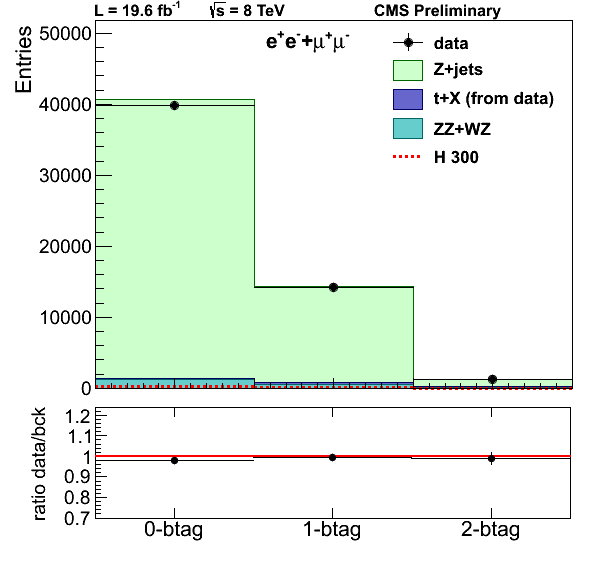
\includegraphics[width=0.49\textwidth]{plots/extra/NBTAG_ll.png}
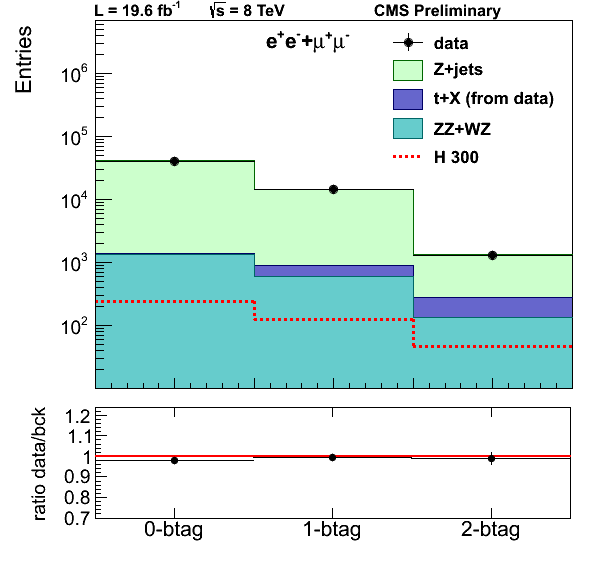
\includegraphics[width=0.49\textwidth]{plots/extra/LOGNBTAG_ll.png}
\caption{Number of events in each btag category after full
selection, for the electron and muon channel combined, in linear (left) and logarithmic scales (right).
Dots indicate data, pale green histogram corrected Z+jets simulation,
light blue simulated diboson background and dark blue $\ttbar$ events from data (which
includes single top, WW, $\Zo\to\TT$+jets).
}
\label{fig:nbtags}
\end{center}
\end{figure}

\vspace*{-5mm}
\begin{figure}[h]
\begin{center}
%% 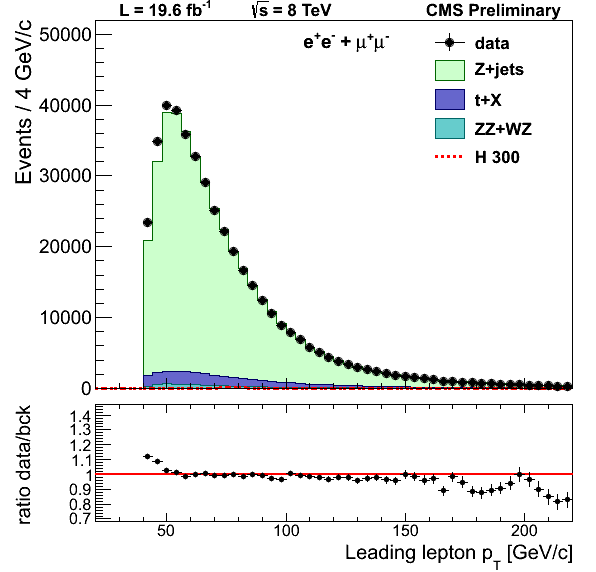
\includegraphics[width=0.32\textwidth]{plots/extra/h_ll_lep_pt0.png}
%% 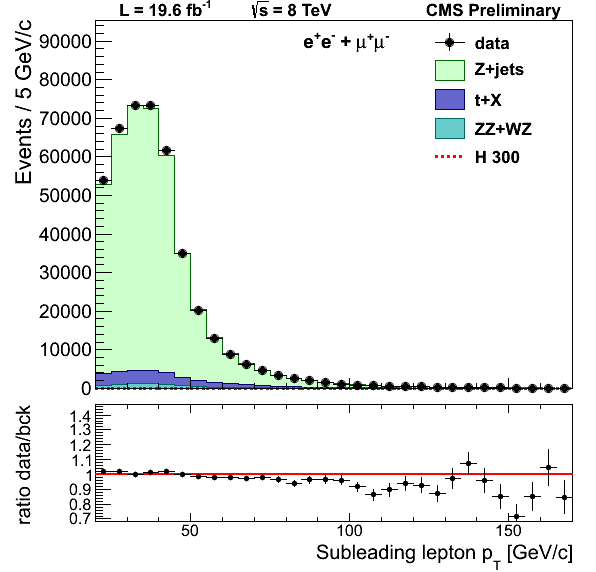
\includegraphics[width=0.32\textwidth]{plots/extra/h_ll_lep_pt1.png} \\
%% 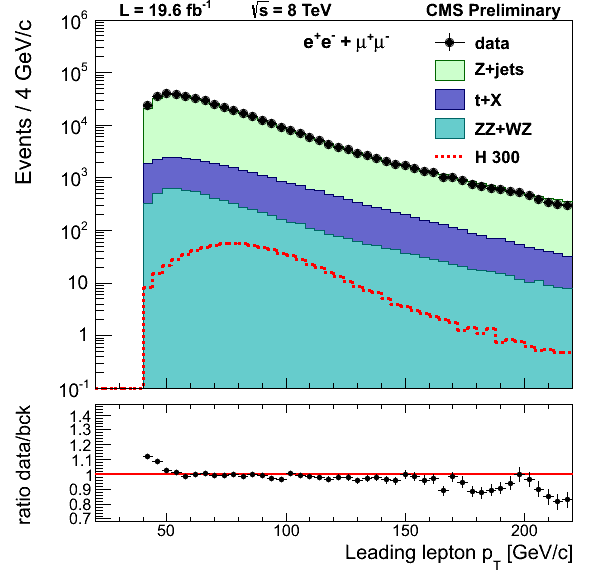
\includegraphics[width=0.32\textwidth]{plots/extra/lh_ll_lep_pt0.png}
%% 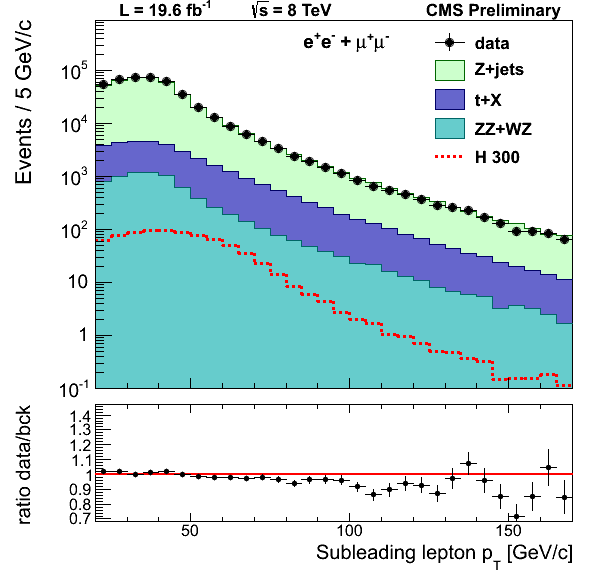
\includegraphics[width=0.32\textwidth]{plots/extra/lh_ll_lep_pt1.png}
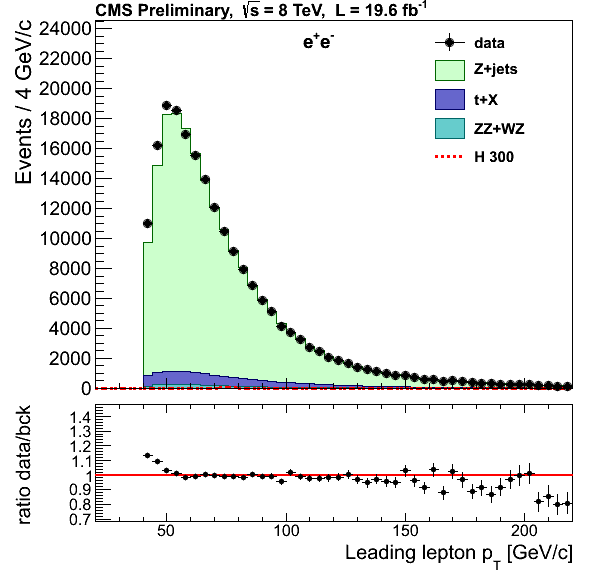
\includegraphics[width=0.32\textwidth]{plots/extra/h_ee_lep_pt0.png}
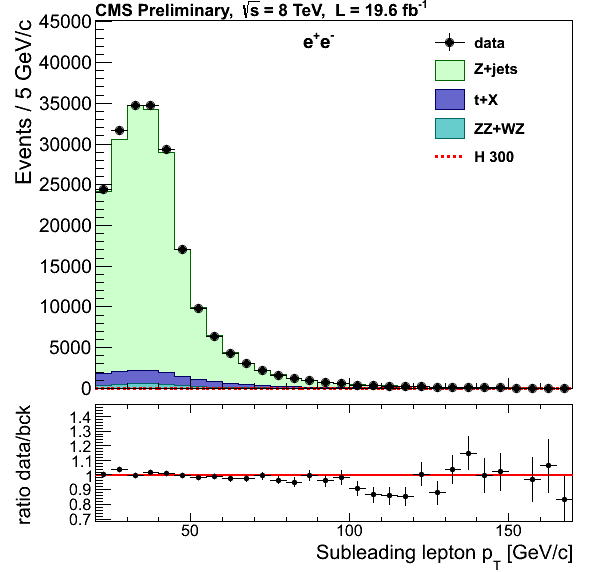
\includegraphics[width=0.32\textwidth]{plots/extra/h_ee_lep_pt1.png} \\
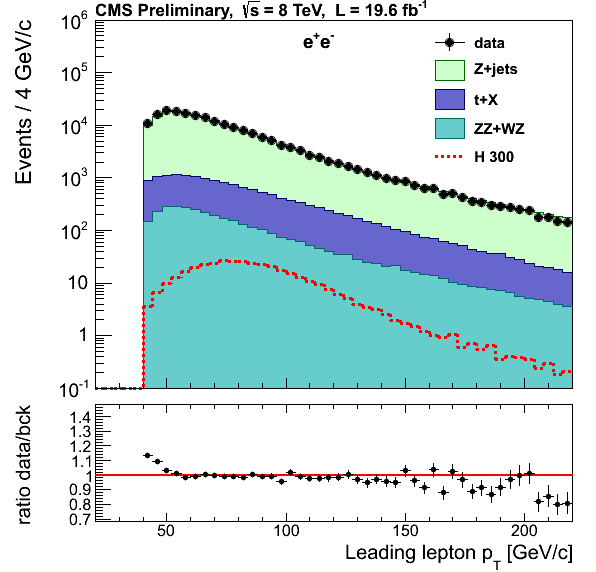
\includegraphics[width=0.32\textwidth]{plots/extra/lh_ee_lep_pt0.png}
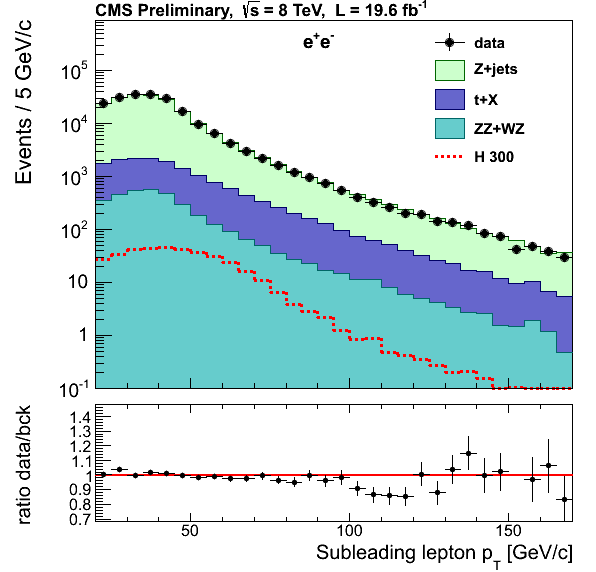
\includegraphics[width=0.32\textwidth]{plots/extra/lh_ee_lep_pt1.png}
\caption{Distributions of the $\pt$ --in linear (upper) and logarithmic scales (lower)--
of the leading (left) and subleading electron (right) after preselection cuts.
Dots indicate data, pale green histogram corrected Z+jets simulation,
light blue simulated diboson background and dark blue $\ttbar$ events from data (which
includes single top, WW, $\Zo\to\TT$+jets).
}
\label{fig:lepptele}
\end{center}
\end{figure}

\vspace*{-5mm}
\begin{figure}[h]
\begin{center}
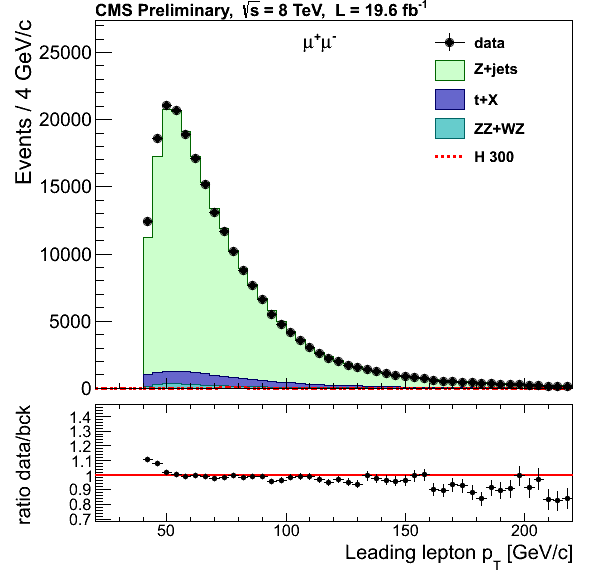
\includegraphics[width=0.32\textwidth]{plots/extra/h_mm_lep_pt0.png}
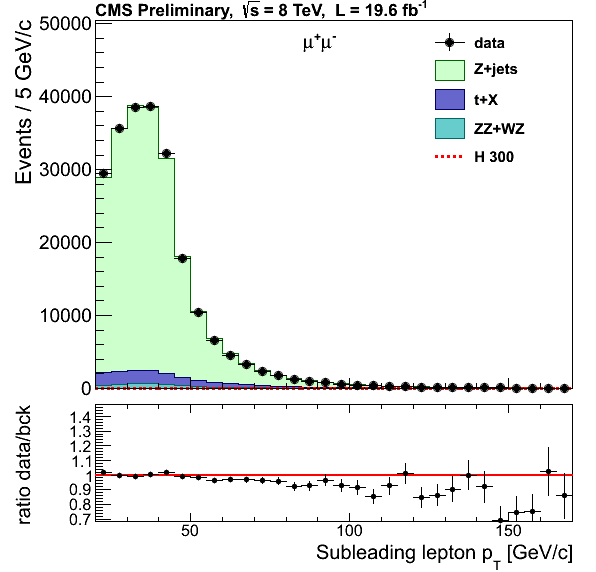
\includegraphics[width=0.32\textwidth]{plots/extra/h_mm_lep_pt1.png} \\
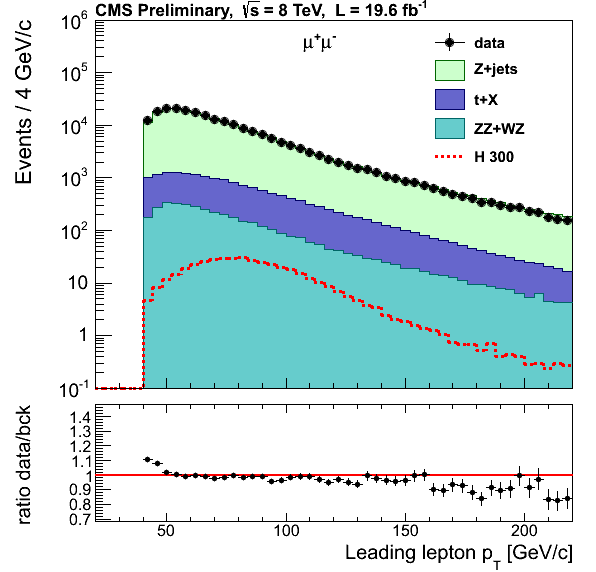
\includegraphics[width=0.32\textwidth]{plots/extra/lh_mm_lep_pt0.png}
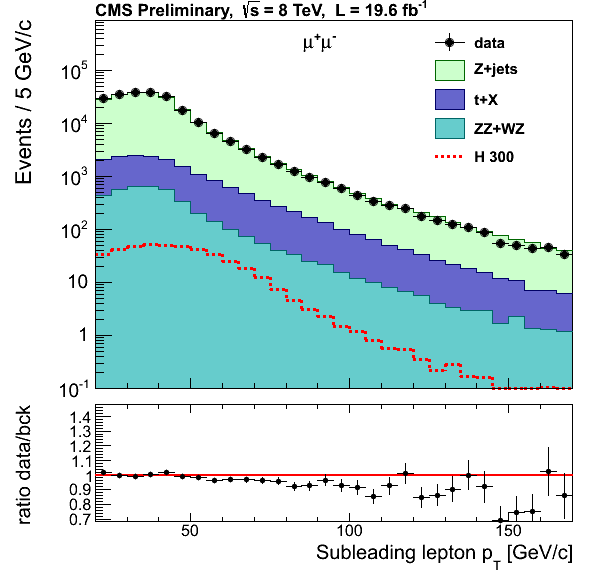
\includegraphics[width=0.32\textwidth]{plots/extra/lh_mm_lep_pt1.png}
\caption{Distributions of the $\pt$ --in linear (upper) and logarithmic scales (lower)--
of the leading (left) and subleading muon (right) after preselection cuts.
Dots indicate data, pale green histogram corrected Z+jets simulation,
light blue simulated diboson background and dark blue $\ttbar$ events from data (which
includes single top, WW, $\Zo\to\TT$+jets).
}
\label{fig:lepptmuon}
\end{center}
\end{figure}

\begin{figure}[h]
\begin{center}
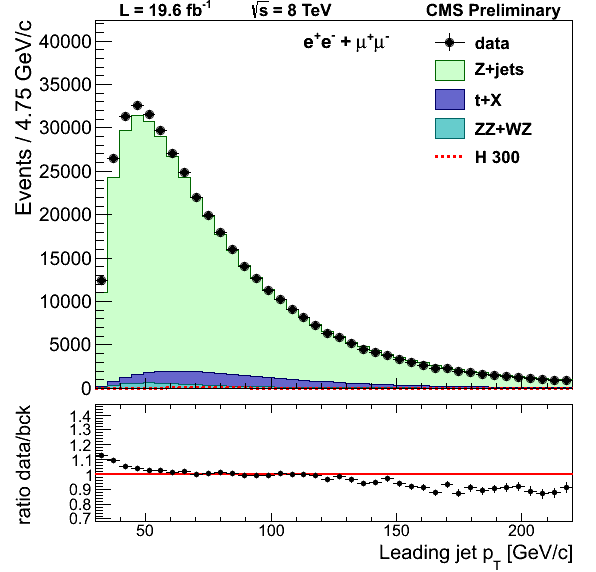
\includegraphics[width=0.32\textwidth]{plots/extra/h_ll_jet_pt0.png}
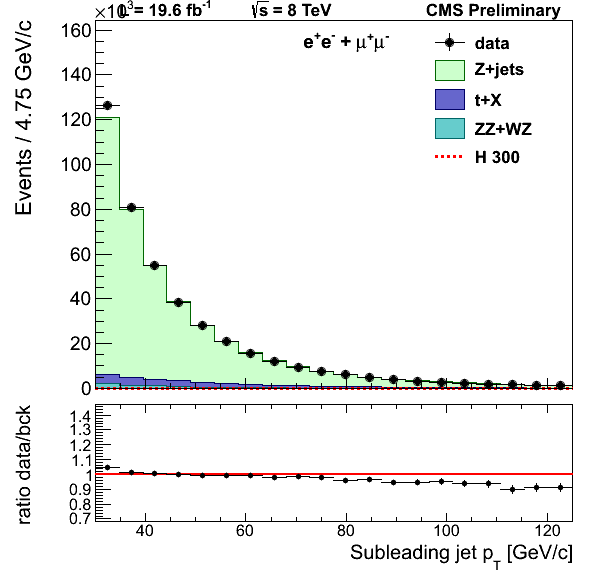
\includegraphics[width=0.32\textwidth]{plots/extra/h_ll_jet_pt1.png} \\
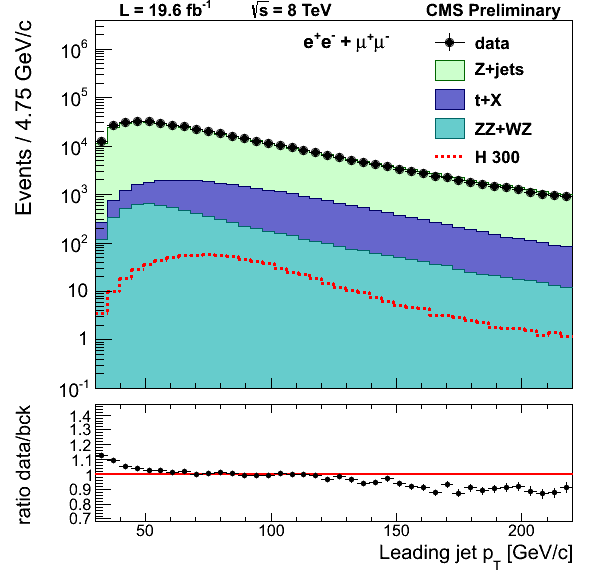
\includegraphics[width=0.32\textwidth]{plots/extra/lh_ll_jet_pt0.png}
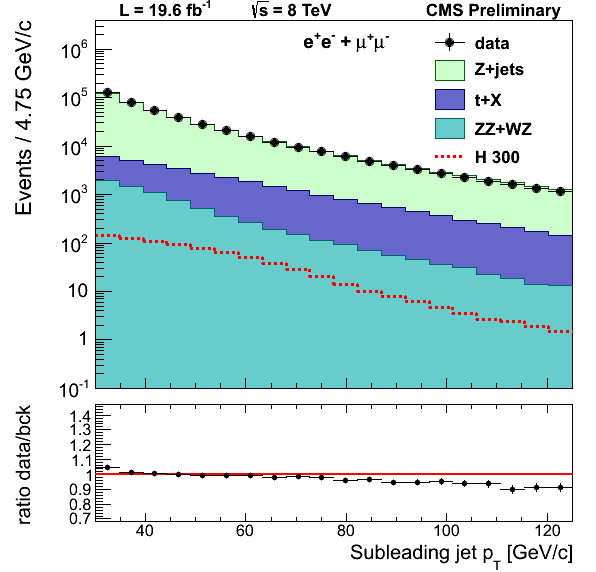
\includegraphics[width=0.32\textwidth]{plots/extra/lh_ll_jet_pt1.png}
\caption{Similar distributions for the leading (left) and subleading jet (right).}
\label{fig:jetpt}
\end{center}
\end{figure}


%\chapter{Checks on the likelihood discriminant}
%\label{sec:costhetastar}
%

The lower-right plot in Figure~\ref{helicityDistDataMCnoLDcut} shows a discrepancy at low LD values.
To identify the source of this discrepancy and quantify the impact on the signal, we have studied
the distributions of the helicity angles before the LD cut. The overall agreement is very good in
all the angles, except in the $\cos\theta^\ast$ distribution for Z+jets events at
$|\cos\theta^\ast| > 0.85$. As a cross-check, Figure~\ref{fig:ctsarcut} presents the LD distribution
applying the cut $|\cos\theta^\ast| < 0.85$, compared to the original LD distribution.
After this cut, Z+jets events are rejected with a minimal impact on the signal efficiency, less than 0.5\%,
and the agreement of the MC with data is significantly improved. 

As an alternative cross-check, rather than cutting in $|\cos\theta^\ast|$, we have weigthed the Z+jets MC
to correct for the improper behavior at $|\cos\theta^\ast| > 0.85$. The resulting distributions 
of $\cos\theta^\ast$ and LD, displayed in Figure~\ref{fig:newldplots}, show a good agreement of the MC
with data, in particular in the LD distribution.

This study demonstrates that the disagreement at low LD values is due to a bad modeling of the
$\cos\theta^\ast$ distribution of Z+jets events at $|\cos\theta^\ast| > 0.85$,
which has a negligible impact on the signal, giving confidence in the analysis.
%%%%%%%%%
\begin{figure}[h]
\centering
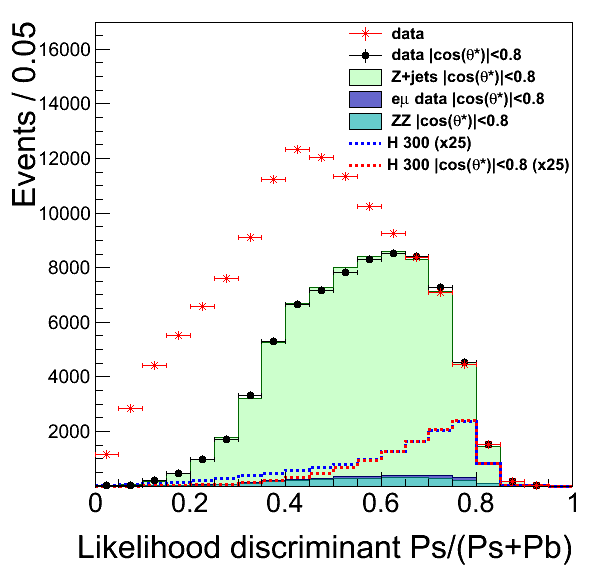
\includegraphics[width=0.49\textwidth]{plots/LD_CUT_ctSTAR.png}
\caption{LD distribution for data (black dots), background (coloured histrograms), and
signal (dashed red line, $\times 25$) events that pass the cut  $|\cos\theta^\ast| < 0.85$.
Uncut distributions for data (red dots) and signal (dashed blue line, $\times 25$) are also
displayed for comparison.
}
\label{fig:ctsarcut}
\end{figure}

\begin{figure}[h]
\centering
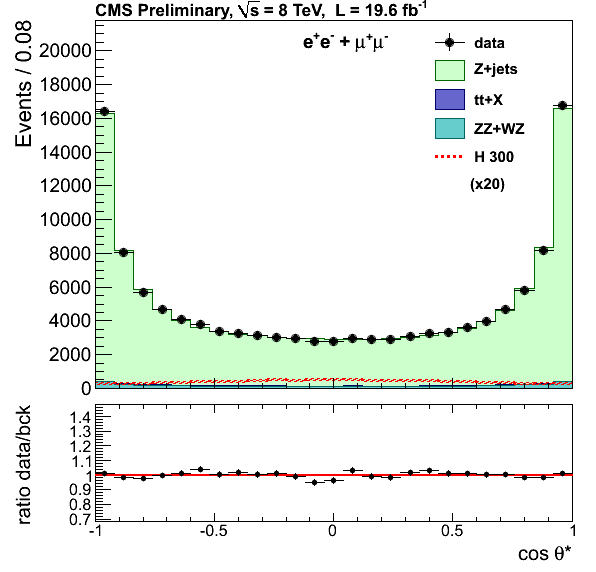
\includegraphics[width=0.49\textwidth]{plots/h_ll_cts_weighted.png}
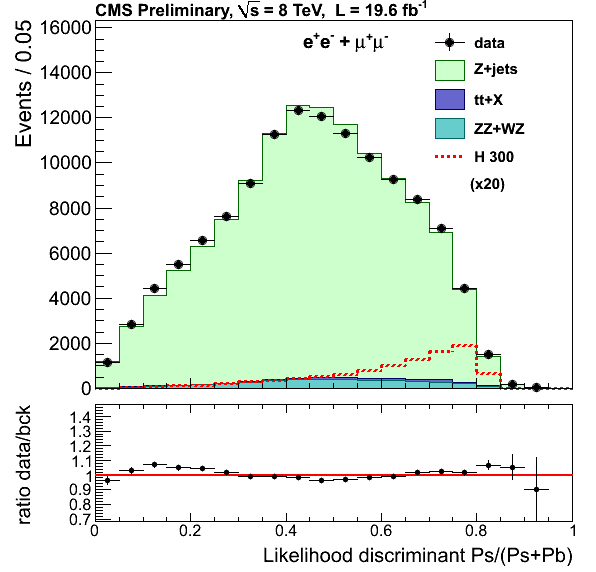
\includegraphics[width=0.49\textwidth]{plots/h_ll_ld_weighted.png}
\caption{$\cos\theta^\ast$ and LD distributionis for data (balck dots), background (coloured histrograms), and
signal (dashed red line, $\times 20$) events. The Z+jets MC is weighted to match the $\cos\theta^\ast$
distribution in data.
}
\label{fig:newldplots}
\end{figure}


\chapter{EXPECTED SIGNAL AND BACKGROUND EVENTS PER BTAG CATEGORY}
\label{sec:numberevents}

Tables~\ref{table:windowYields0tag},~\ref{table:windowYields1tag}, and~\ref{table:windowYields2tag}, list 
the numbers of signal and background events expected for 19.6 $\text{fb}^{-1}$
in the mass range $[\MH -6\%, \MH+10\%]$ in the three btag categories, separately for the $\MM jj$
and $\EE jj$ channels (denoted $\mu\mu$ and ee, respectively).

\begin{table}[h!]
\caption{Expected yields in the 0-btag category.}
\label{table:windowYields0tag}
\centering
\begin{tabular}{|c|c|c|c|c|c|c|c|c|c|c|} \hline
    $\MH~(\GeVcc)$   & \multicolumn{2}{c|}{signal}      & \multicolumn{2}{c|}{Z+jets} & \multicolumn{2}{c|}{e$\mu$ data} & \multicolumn{2}{c|}{diboson} & \multicolumn{2}{c|}{total background} \\ \cline{2-11}
                 & $\mu\mu$ & ee &  $\mu\mu$ &  ee &  $\mu\mu$ &  ee &  $\mu\mu$ &  ee & $\mu\mu$ & ee \\\hline
    250  &  90.0 & 80.4 & 6160.5 & 5312.2 &24 & 19  &201.7 & 175.6 &6386.3 & 5506.7 \\
    300  &  90.0 & 80.6 & 3334.3 & 2800.3 & 11 & 9  &121.1 & 106.6 &3466.6 & 2915.7 \\
    400  &  82.6 & 73.5 & 1254.4 & 1065.9 & 1 & 0   & 55.9 & 49.3 & 1310.9 & 1115.6 \\
    500 &33.4 & 30.2 &429.0 & 381.9 &1 & 1  &23.9 & 20.4 &454.0 & 403.2 \\
    600&11.9 & 10.5 &179.3 & 152.3 &0 & 0  &11.3 & 10.8 &190.6 & 163.2 \\\hline
\end{tabular}
\end{table}

\begin{table}[h!]
\caption{Expected yields in the 1-btag category.}
\label{table:windowYields1tag}
\centering
\begin{tabular}{|c|c|c|c|c|c|c|c|c|c|c|} \hline
    $\MH~(\GeVcc)$   & \multicolumn{2}{c|}{signal}      & \multicolumn{2}{c|}{Z+jets} & \multicolumn{2}{c|}{e$\mu$ data} & \multicolumn{2}{c|}{diboson} & \multicolumn{2}{c|}{total background} \\ \cline{2-11}
                 & $\mu\mu$ & ee &  $\mu\mu$ &  ee &  $\mu\mu$ &  ee &  $\mu\mu$ &  ee & $\mu\mu$ & ee \\\hline
    250 & 44.7 & 40.1 &2124.7 & 1779.0 &87 & 68  &89.7 & 74.2 &2301.2 & 1921.4 \\
    300 & 46.8 & 40.8 &1174.5 & 987.0 &33.0 & 25  &60.8 & 49.1 &1268.3 & 1062.1 \\
    400&45.0 & 40.8 &459.8 & 406.7 &6 & 5  &26.9 & 24.1 &492.9 & 435.7 \\
    500&18.9 & 17.0 &181.1 & 155.8 &1 & 0  &13.9 & 10.1 &195.5 & 166.3 \\
    600 & 7.0 & 6.4 &80.9 & 61.4  &0 & 0  &6.5 & 5.5 &87.4 & 66.9 \\\hline
\end{tabular}
\end{table}

\begin{table}[h!]
\caption{Expected yields in the 2-btag category.}
\label{table:windowYields2tag}
\centering
\begin{tabular}{|c|c|c|c|c|c|c|c|c|c|c|} \hline
    $\MH~(\GeVcc)$   & \multicolumn{2}{c|}{signal}      & \multicolumn{2}{c|}{Z+jets} & \multicolumn{2}{c|}{e$\mu$ data} & \multicolumn{2}{c|}{diboson} & \multicolumn{2}{c|}{total background} \\ \cline{2-11}
                 & $\mu\mu$ & ee &  $\mu\mu$ &  ee &  $\mu\mu$ &  ee &  $\mu\mu$ &  ee & $\mu\mu$ & ee \\\hline
    250&15.6 & 14.8 &180.9 & 138.6 &42 & 33  &18.7 & 16.4 &241.7 & 188.0 \\
    300&18.5 & 16.0 &91.2 & 70.9 &28 & 22  &12.2 & 11.7 &131.4 & 104.6 \\
    400&19.8 & 16.8 &32.2 & 24.6 &1 & 0  &7.0 & 5.3 &39.7 & 30.4 \\
    500&8.2 & 7.5 &9.6 & 8.9 &0 & 0  &2.7 & 2.5 &12.3 & 11.4 \\
    600&3.0 & 2.8 &5.6 & 4.5 &0 & 0  &1.7 & 1.5 &7.3 & 6.0 \\\hline
\end{tabular}
\end{table}


\chapter{DETERMINATION OF $\ttbar$ BACKGROUND FROM DATA}
\label{sec:appttbar}

In the analysis, the $\Pqt \Paqt$ background is estimated from data. Additional
plots supporting the robustness of the procedure are presented below.
The comparison of $\EM$ and $(\EE+\MM)$ dsitributions using Powheg + Pythia top MC shows
an excellent agreement, as depicted in Figure~\ref{figap:emumc1}
for several variables after different steps of the selection. A similar agreement
is observed in Figure~\ref{figap:emudata1}, which compares the 2012 $\EM$ data to Powheg + Pythia top MC.
Figure~\ref{figap:emu_ll_comp_met} displays the MET significance distribution
for dilepton data compared to the sum of Drell-Yan Monte Carlo
plus $\EM$ data for events with two b-tags (1 JPM + 1 JPL), and the dijet
invariant mass (right) for $\EE + \MM$ and $\EM$ data for events outside the leptonic $Z$ mass window,
show again very good agreement.

\begin{figure}[!htb]
  \centerline{
    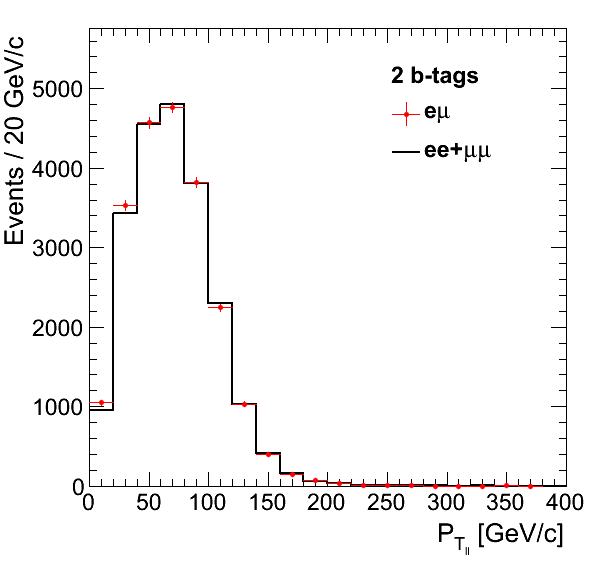
\includegraphics[width=0.43\textwidth]{plots/emu_mc_ZllPt_5}
    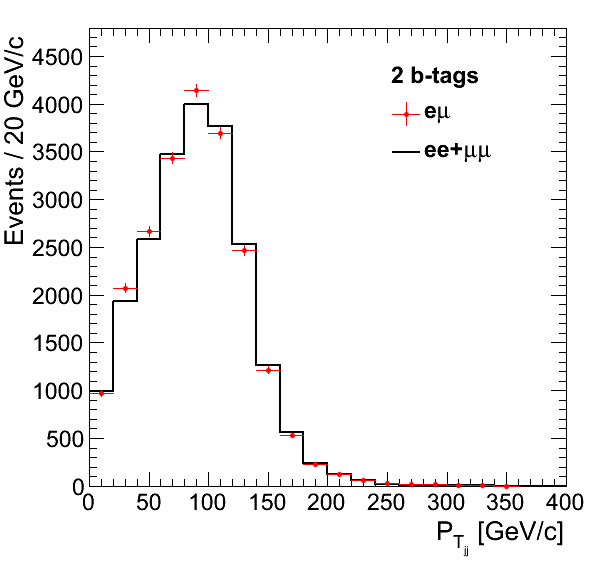
\includegraphics[width=0.43\textwidth]{plots/emu_mc_ZjjPt_5}
  }
  \centerline{
    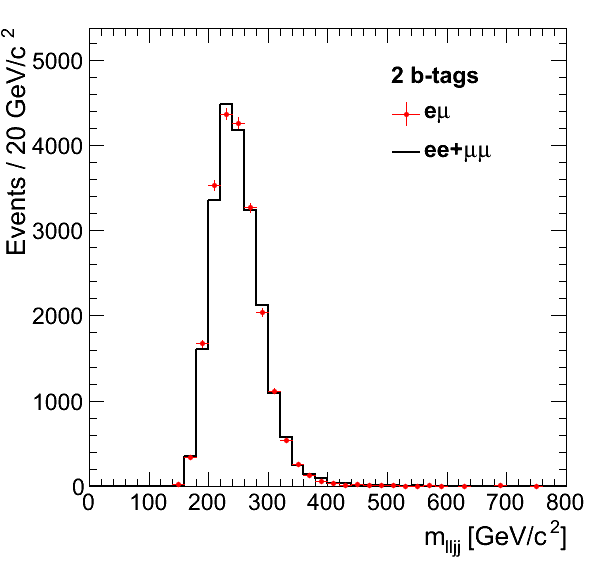
\includegraphics[width=0.43\textwidth]{plots/emu_mc_HiggsMass_5}
    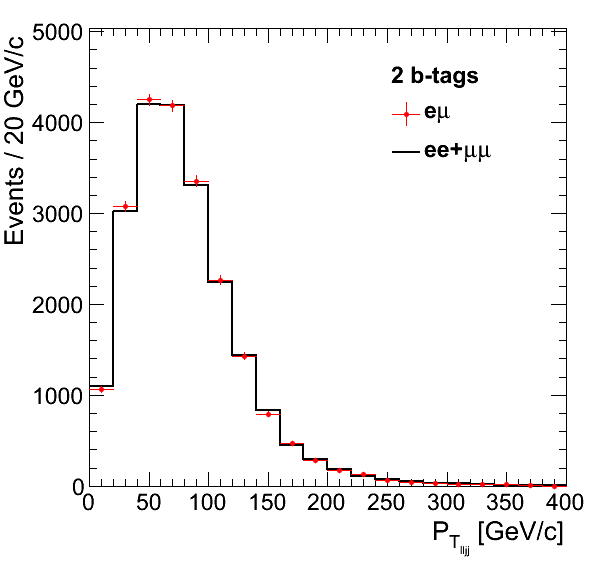
\includegraphics[width=0.43\textwidth]{plots/emu_mc_HiggsPt_5}
  }
  \caption{\label{figap:emumc1} Powheg + Pythia top MC $\EM$ to
    $(\EE+\MM)$ comparison for several variables after different
    steps of the selection, as specified in the legends. Top:
    dilepton (left) and dijet transverse momentum (right). Bottom:
    dilepton + dijet ``Higgs'' invariant mass (left) and transverse
    momentum (right).}
\end{figure} 

\begin{figure}[!htb]
  \centerline{
    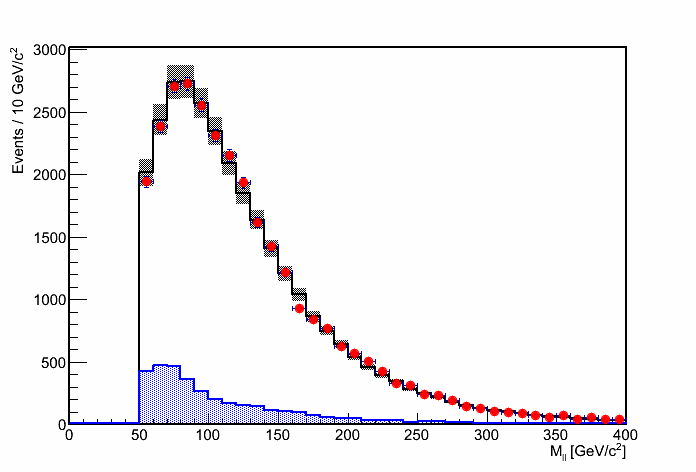
\includegraphics[width=0.49\textwidth]{plots/emu_zllm1_0}
    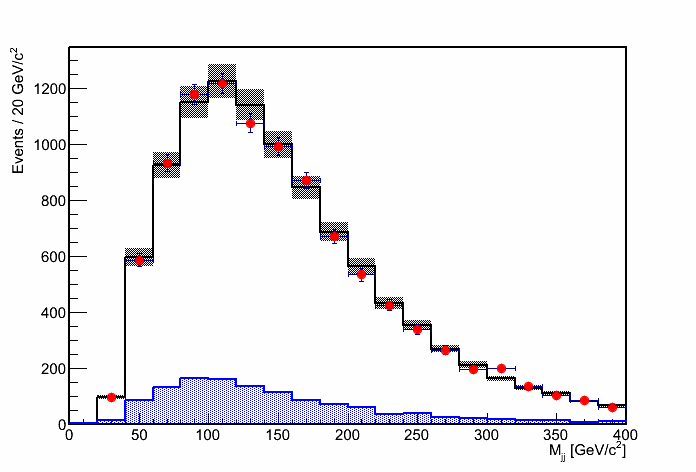
\includegraphics[width=0.49\textwidth]{plots/emu_zjjm2_0}
  }
  \centerline{
    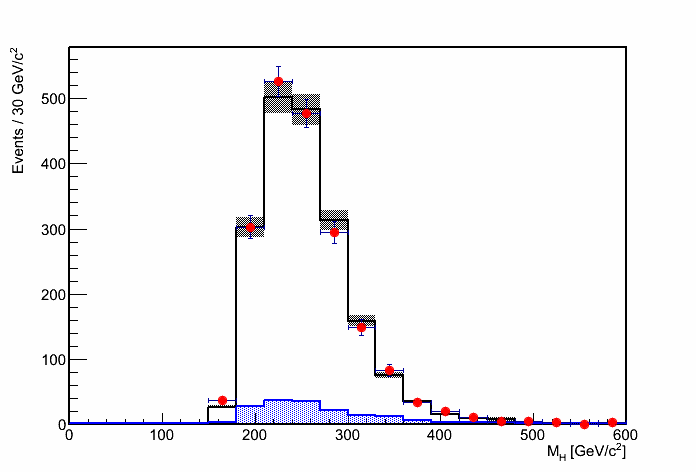
\includegraphics[width=0.49\textwidth]{plots/emu_hm3_1}
    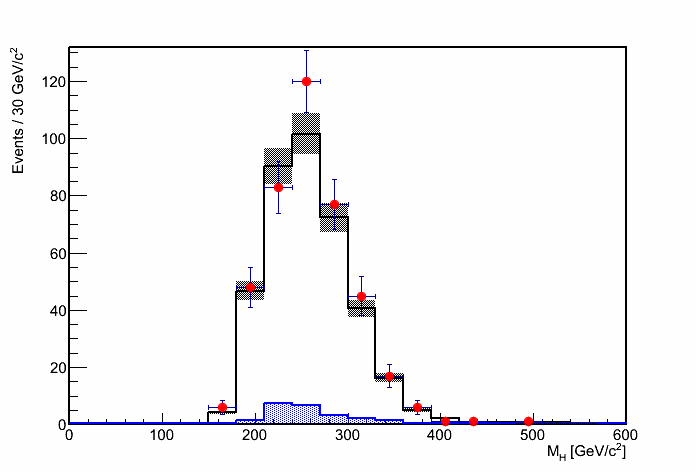
\includegraphics[width=0.49\textwidth]{plots/emu_hm3_3}
  }
  \caption{\label{figap:emudata1}Comparison of 2012 $\EM$ data to
    Powheg + Pythia top MC, corresponding to an integrated luminosity
    of 19.6 fb$^{-1}$. Red dots are $\EM$ data; white histogram top
    Monte Carlo; blue histogram other small backgrounds.  Top:
    dilepton invariant mass (left) and dijet invariant mass
    (right). Bottom: ``Higgs'' invariant mass for events with 1
    JPL b-tag (left), and two (1 JPM + 1 JPL) b-tags and MET
    significance $< 10$ (right).}
\end{figure}

Next, the data-driven evaluation of the $\Pqt \Paqt$ background is compared to an alternative
method based on top simulation only. 
Figure~\ref{figap:emudata2} compares the previous $\EM$ data distributions to the prediction of
Powheg + Pythia top MC normalized to the NLO $\Pqt \Paqt$ cross-section.
The gray area represents the systematic error (including luminosity, lepton trigger and ID efficiencies,
b-tagging efficiency, mistag efficiency, and pile-up uncertainties; no contribution from normalization) of the MC
prediction. With the 19.6~\fbinv{}, the statistical errors of the $\EM$ data points compare well
to the size of the gray boxes. In addition, the $\Pqt \Paqt$ MC underestimates the normalization of the
$\EM$ data by $20\%$ before b-tagging ($12\%$ for events with  2 b-tagged jets). Based on this comparison
we choose to use the data-driven estimation.

\begin{figure}[!htb]
  \centerline{
    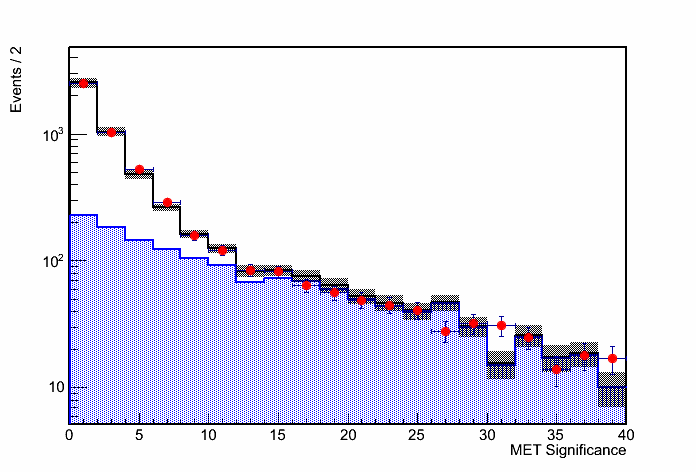
\includegraphics[width=0.55\textwidth]{plots/emu_mets1l_2dy}
    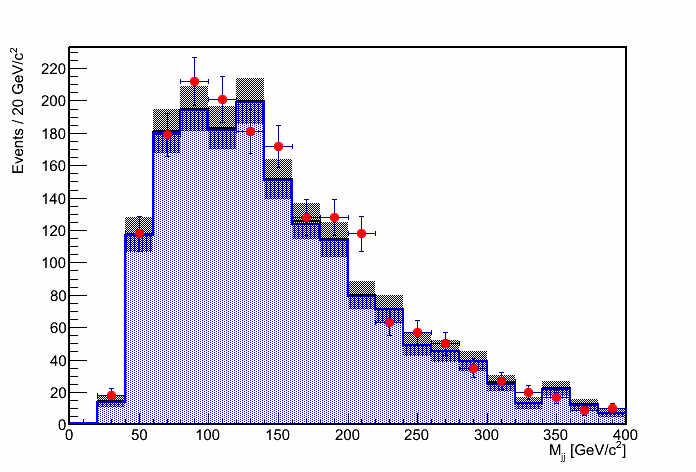
\includegraphics[width=0.55\textwidth]{plots/emu_zjjm2_2dy_side}
  }
  \caption{ \label{figap:emu_ll_comp_met} MET significance distribution
    for dilepton data compared to the sum of Drell-Yan Monte Carlo
    plus $\EM$ data for events with two btags (left).
    Dijet invariant mass (right) for $\EE + \MM$ and $\EM$
    data for events outside the leptonic $Z$ mass window, with two
    b-tags, and MET significance $>$ 8. Other cuts are
    detailed in the text.
    Red dots are $\EE+\MM$ data; white
    histogram Drell Yan Monte Carlo; blue histogram $\EM$ data (plus
    other small backgrounds).}

\end{figure}

\begin{figure}[!htb]
  \centerline{
    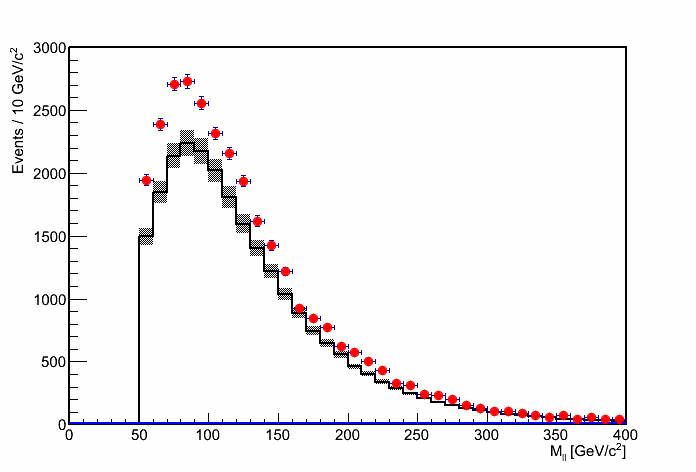
\includegraphics[width=0.49\textwidth]{plots/emu_zllm1_4}
    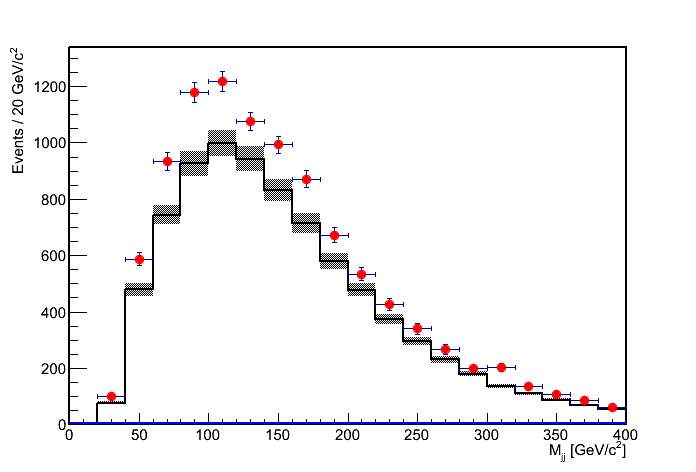
\includegraphics[width=0.49\textwidth]{plots/emu_zjjm2_4}
  }
  \centerline{
    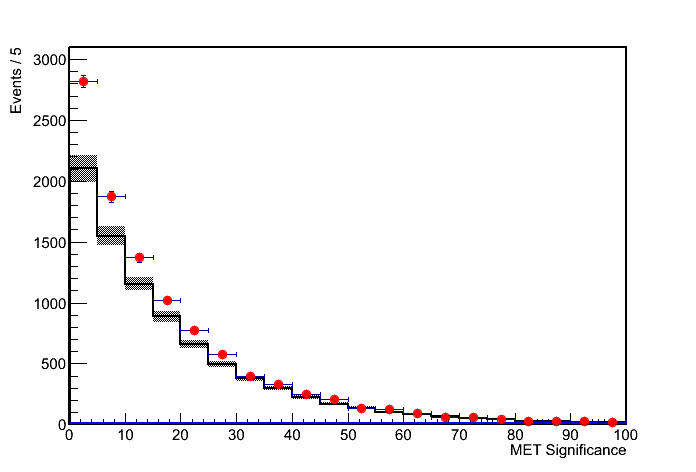
\includegraphics[width=0.49\textwidth]{plots/emu_mets2_4}
    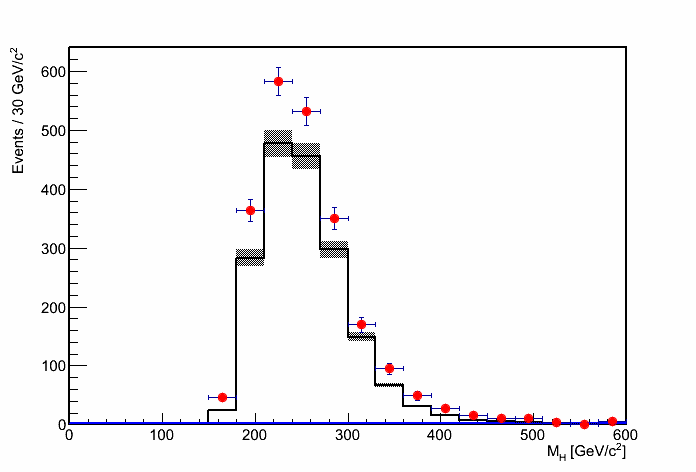
\includegraphics[width=0.49\textwidth]{plots/emu_hm3_4}
  }
  \caption{\label{figap:emudata2}Comparison of 2012 $\EM$ data to
    Powheg + Pythia top MC normalized to the $\Pqt \Paqt$ NLO cross-section.
    Red dots are $\EM$ data; white histogram top Monte Carlo. Top:
    dilepton invariant mass (left) and dijet invariant mass
    (right). Bottom: MET significance (left), and ``Higgs'' invariant
   mass  (right).}
\end{figure}





\chapter{MASS DISTRIBUTIONS FOR THE ELECTRON AND MUON CHANNELS}
\label{sec:emuratios}

The $\mlljj$ distributions, depicted in Figure~\ref{fig:emuratios}
for the electron and muon channels, display an
excellent agreement both in the $m_{jj}$ sideband and signal regions.

\begin{figure}[htb]
\begin{center}
\centerline{
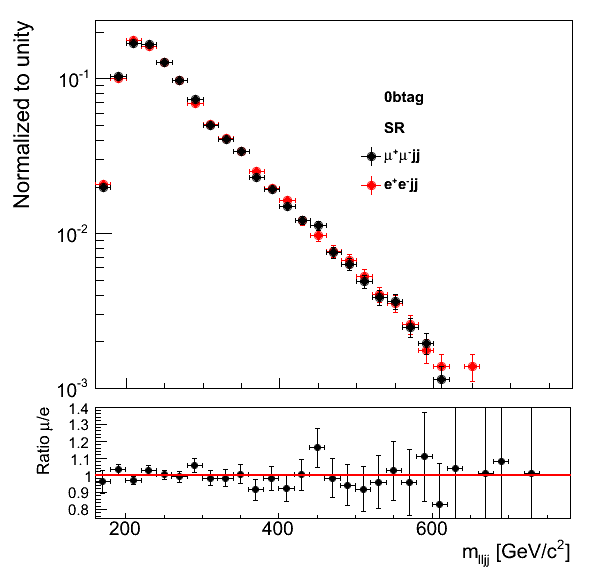
\includegraphics[width=0.33\textwidth]{plots/mH_lim20_0btag_NORM_LOG.png}
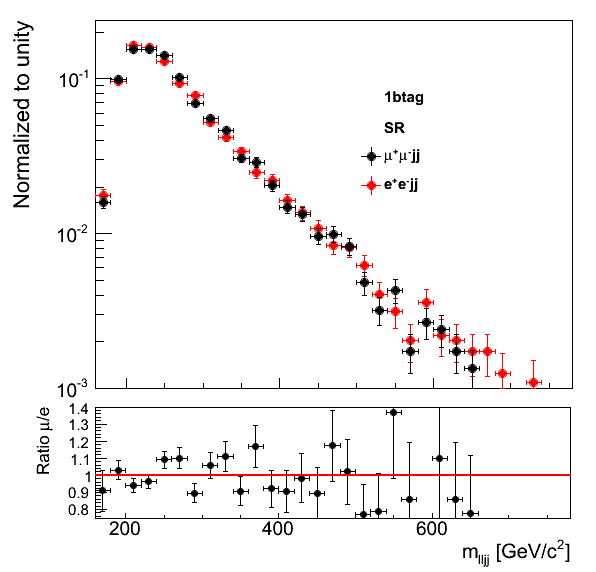
\includegraphics[width=0.33\textwidth]{plots/mH_lim20_1btag_NORM_LOG.png}
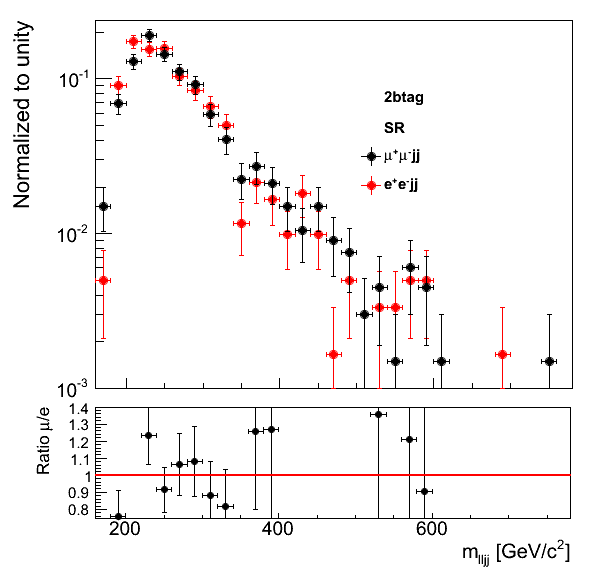
\includegraphics[width=0.33\textwidth]{plots/mH_lim20_2btag_NORM_LOG.png}
}
\centerline{
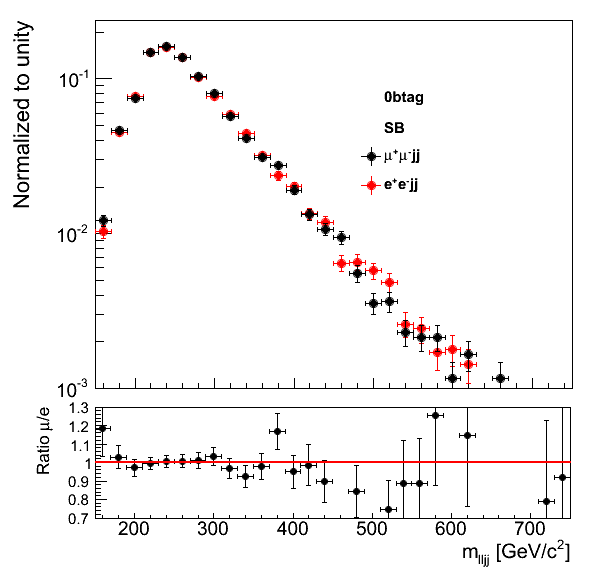
\includegraphics[width=0.33\textwidth]{plots/mH_lim20_0btag-SB_NORM_LOG.png}
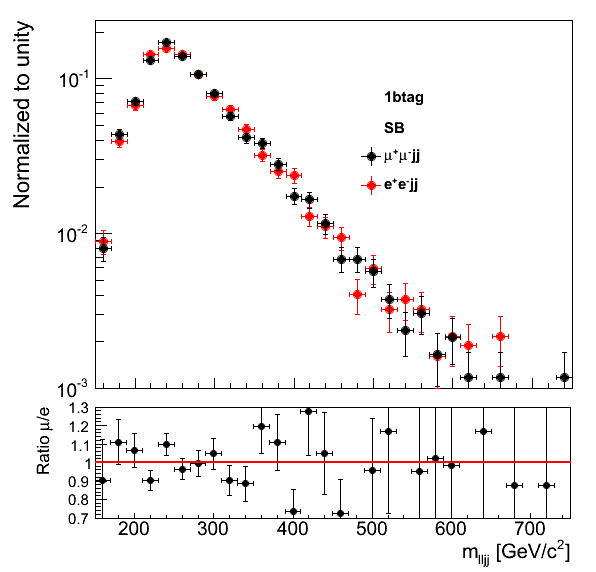
\includegraphics[width=0.33\textwidth]{plots/mH_lim20_1btag-SB_NORM_LOG.png}
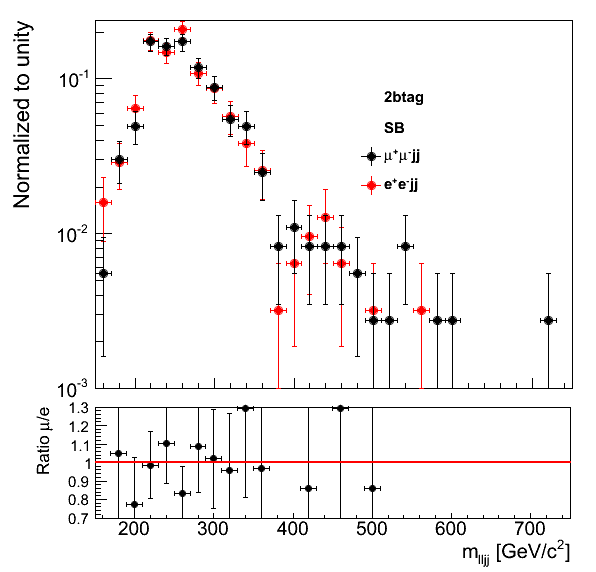
\includegraphics[width=0.33\textwidth]{plots/mH_lim20_2btag-SB_NORM_LOG.png}
}
\caption{Mass distributions of the $\LL jj$ system for events in the
electron and muon channels: data in the $m_{jj}$
(top) signal and (bottom) sideband regions.
From left to right, plots
correspond to the 0-, 1-, and 2-btag categories.
}
\label{fig:emuratios}
\end{center}
\end{figure}



\chapter{LIMIT CROSS CHECKS}
\label{sec:cutcount}
Another approach, referred to as \textit{cut-and-count} analysis,
 uses only the number of events selected with a reconstructed Higgs mass in the 
window $[\MH -6\%, \MH+10\%]$. The Higgs cross section limit is determined from the expected number of signal
and background events passing the selections $s$ and $b$ respectively.
%Lower Figure~\ref{fig:limit5fb} shows the same observed  limit on the ratio for the unblinded dataset, using the cut-and-count technique.
%The expectation for the full dataset is also shown in Figure~\ref{fig:limit5fb}~(down).
The results shown in Figure~\ref{fig:cutcount} are compatible with the full results.

\begin{figure}[htbp]
 \begin{center}
 \centerline{
 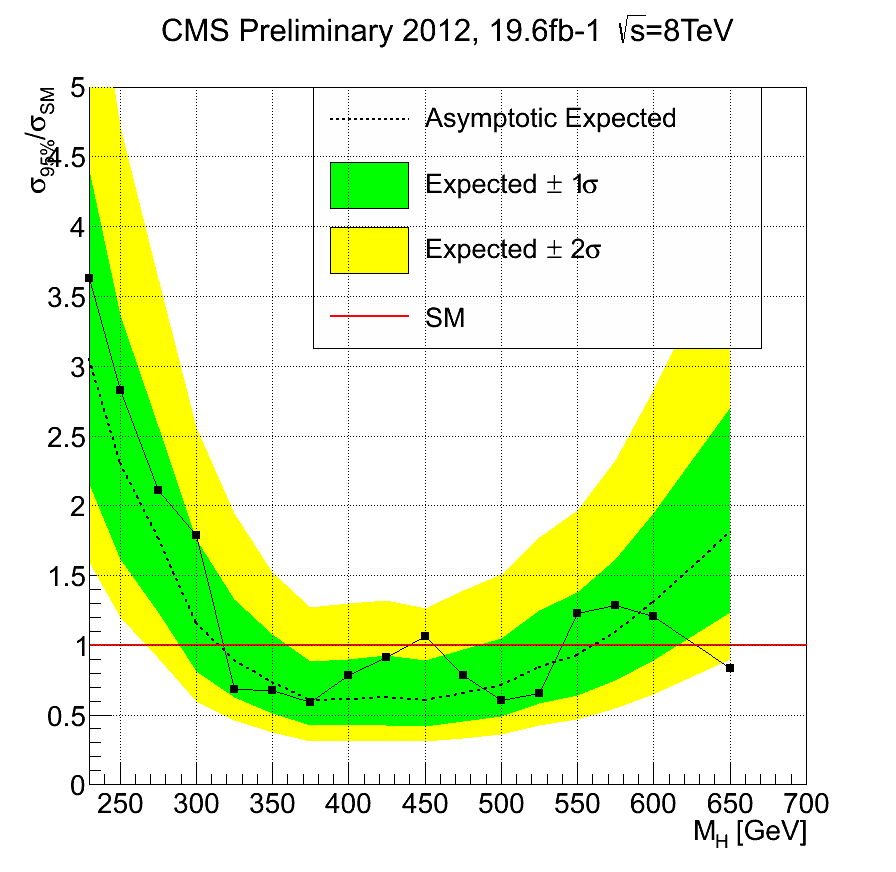
\includegraphics[width=0.49\textwidth]{plots/limit_CiC_unblinded_win0.png}
%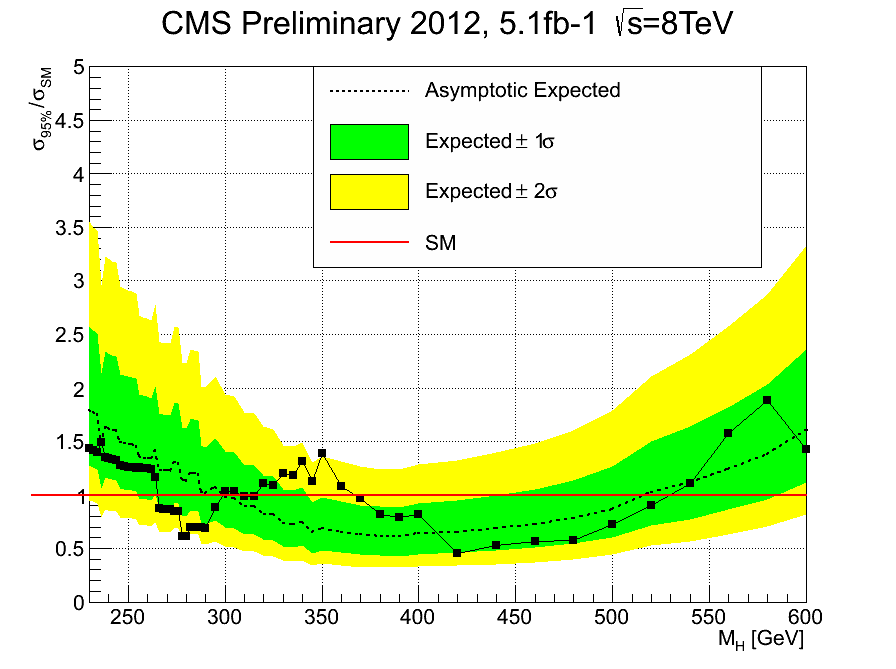
\includegraphics[width=0.49\textwidth]{plots/limit_CiC5_5fb_unblinded.png}
}
\caption{
Observed (solid) and expected (dashed) 95\% CL upper limit
on the ratio of the production cross section to the SM expectation
for the Higgs boson obtained using the \textit{cut-and-count} technique,
which integrates the mass distributions in a
range $[\MH -6\%, \MH+10\%]$ around each Higgs mass hypothesis.
The 68\% and 95\% ranges of expectation
for the background-only model are also shown with green and
yellow bands, respectively.  The solid line at 1 indicates the expectation
for a SM-Higgs-like boson.
}
\label{fig:cutcount}
\end{center}
\end{figure}


%\chapter{Cross Checks requested at Approval}
%\label{sec:approvalxcheck}
%The following cross checks were requested during approval:
\begin{itemize}
\item Take the Z+jets MC sample and define the scale factor based on the
overall number of events after the preselection in the signal dijet mass
window with respect to the sideband mass windows. Apply this constant scale
factor to the differential distribution of 4-body mass in the Z+jets events
in the sideband and see if you reproduce that for the signal region in the
entire mass range.

\item Compare the 4-body mass distributions for the lower and upper sideband in
the data and see if the ratio is constant with the 4-body mass.

\item Make a technical check of the last steps of the analysis, just to be safe.

\item Make the combination with 7 TeV as published (this was a condition at the pre-approval in fact).

\item Consider stopping the analysis at 600 GeV in light of the concerns.

\end{itemize}

\subsection{}

As can be seen in Figure~\ref{fig:clos} the tail is basically the same, implying that there is no issue
in the shape due to jet merging or so. In the low mass region there is a clear
difference, but this has already been studied in the past and it is due to the
bias from the mJJ selection.

However, this is not a closure test as one may think on such: if it is intended to
validate our analysis methodology, it is not the proper test, since this is not
what we do in the analysis (more below). If it is to check that the shapes are
the same, they are not... and we know that: the mllJJ and mJJ variables are not
fully decoupled (specially at low masses) and therefore there are differences.

It should be added that in our analysis we are not taking the shape of the SB
for anything except to validate the MC expectations. The shape in the SB does
not have any influence in the result. It has been relevant of course in the
decision to unblind the analysis, but only that. We are not using it in any way
to infer the shape in the SR for Z+jets (that is what the test above seems to
suggest).
Only the normalization in the SB has some impact on the result.

In our analysis, we are not assuming that the shape from the SB is able to
reproduce the SR. Even if at high masses they agree (because the requirement on
mJJ has smaller influence), we are not using that information.
We are extracting the expected shape from the same SR but the MC and we are
assuming that MC reproduces the SR as well as the SB. In fact today we know that
the MC reproduces the shape in BOTH SB, so assuming it also works in the SR is
the natural thing to do. We have no reason to think that there is something in
the Z-peak region affecting Z+jets that does not affect any of the two SB, one
at lower masses and the other at higher masses.

Furthermore (last but not least), we did not claim that the shape in the MC is
perfectly reproduced and we have a systematic uncertainty. As shown in the
approval talk, we quote a large systematic on the shape that covers by far any
discrepancy observed in the SB regions (plots this morning).
Recall the systematic is really large at high masses.

\begin{figure}[htb]
\centerline{
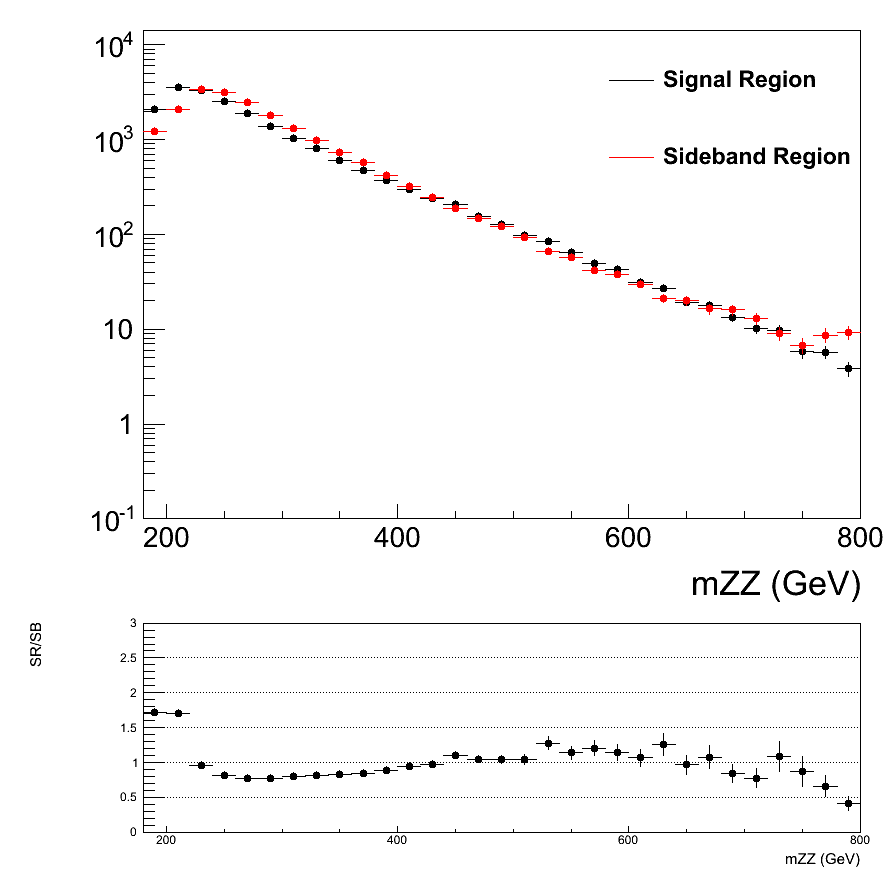
\includegraphics[width=0.33\textwidth]{plots/approvalxchecks/mZZ_SRvsSB_lep0_0btags_Log.png}
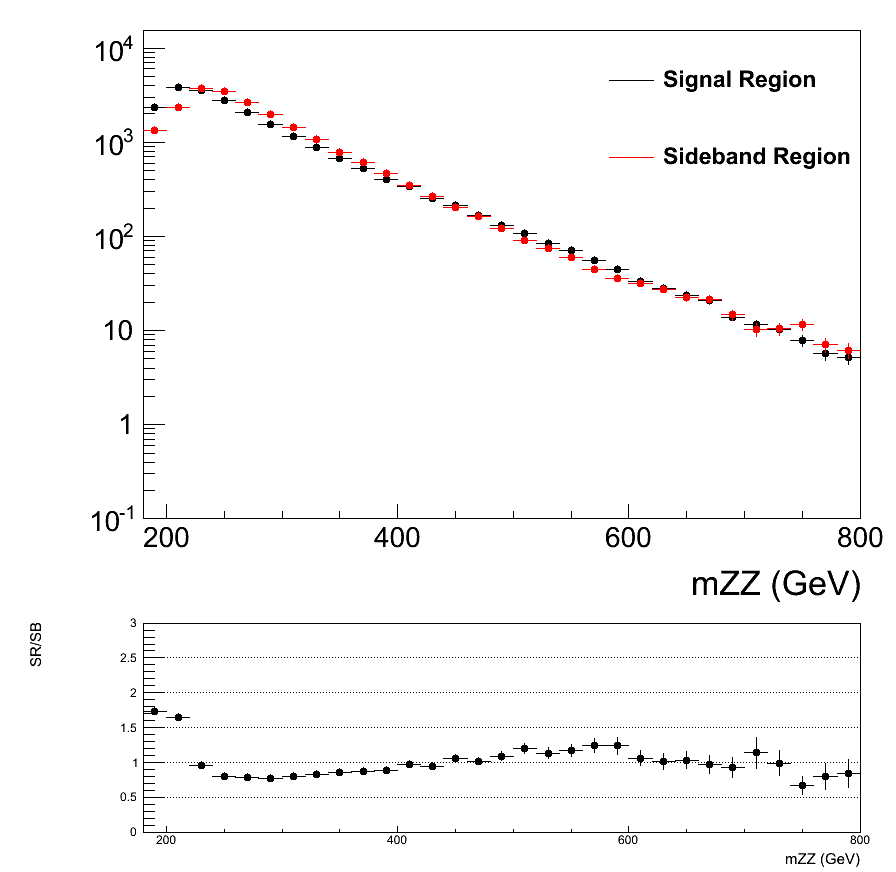
\includegraphics[width=0.33\textwidth]{plots/approvalxchecks/mZZ_SRvsSB_lep1_0btags_Log.png}
}
\centerline{
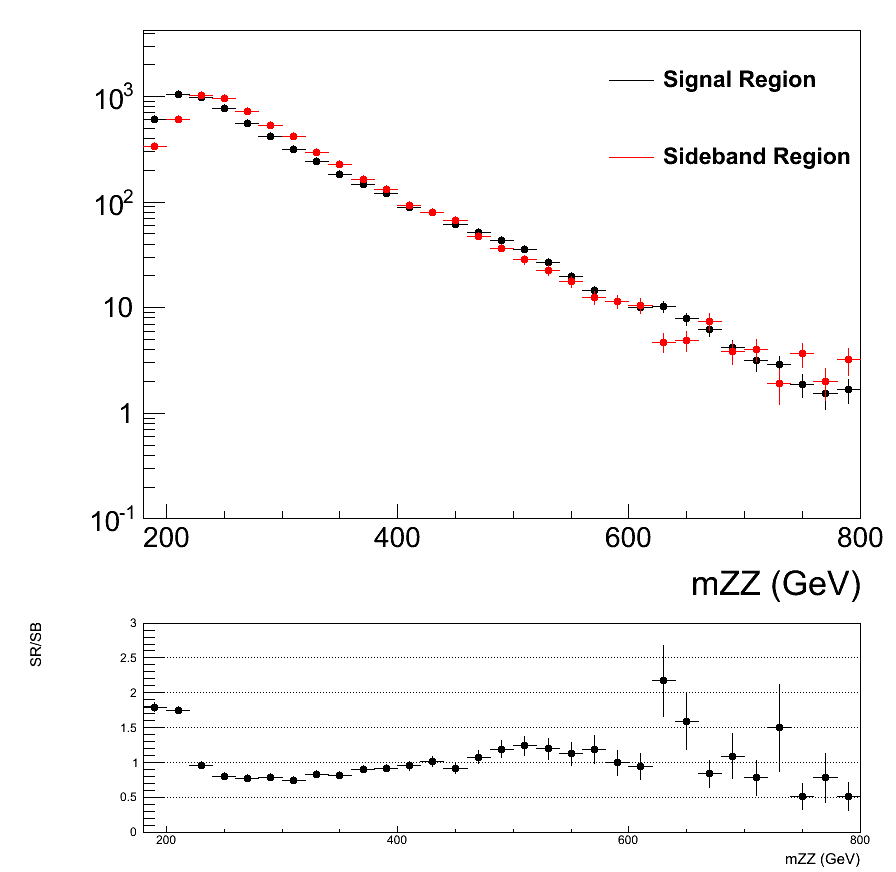
\includegraphics[width=0.33\textwidth]{plots/approvalxchecks/mZZ_SRvsSB_lep0_1btags_Log.png}
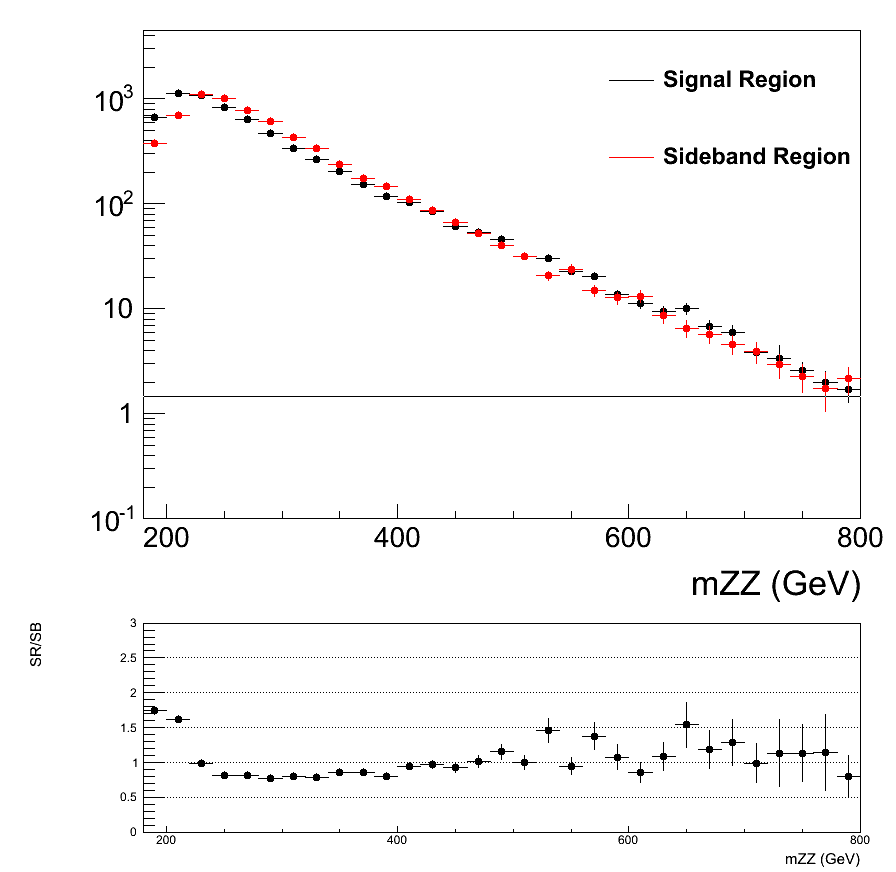
\includegraphics[width=0.33\textwidth]{plots/approvalxchecks/mZZ_SRvsSB_lep1_1btags_Log.png}
}
\centerline{
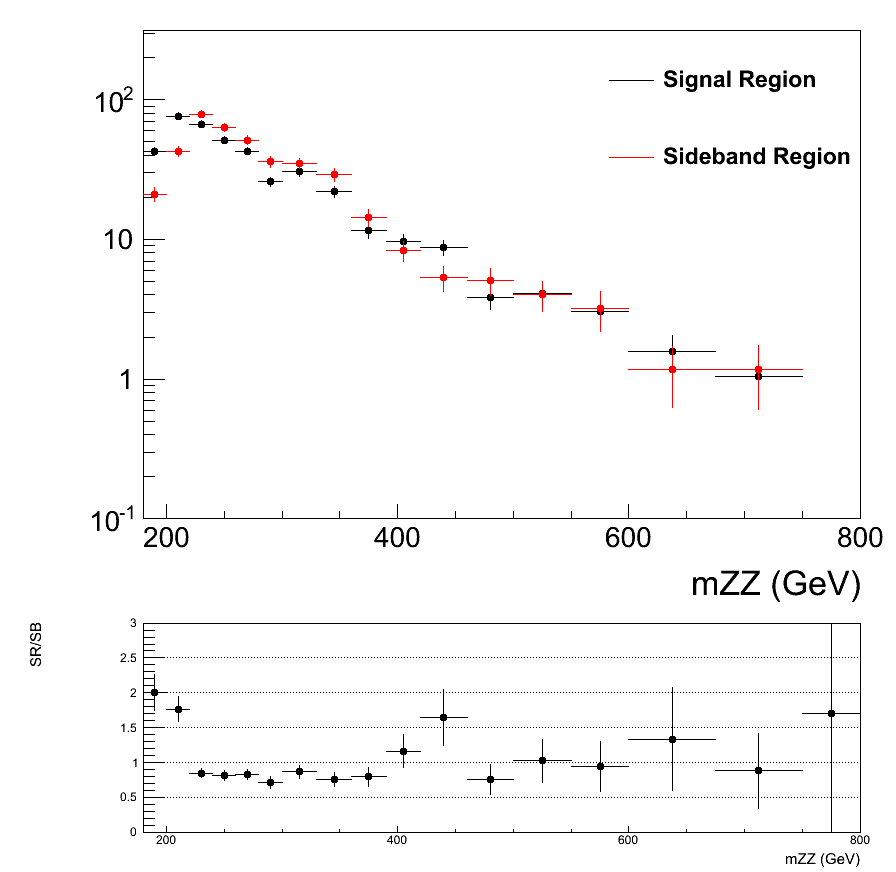
\includegraphics[width=0.33\textwidth]{plots/approvalxchecks/mZZ_SRvsSB_lep0_2btags_Log.png}
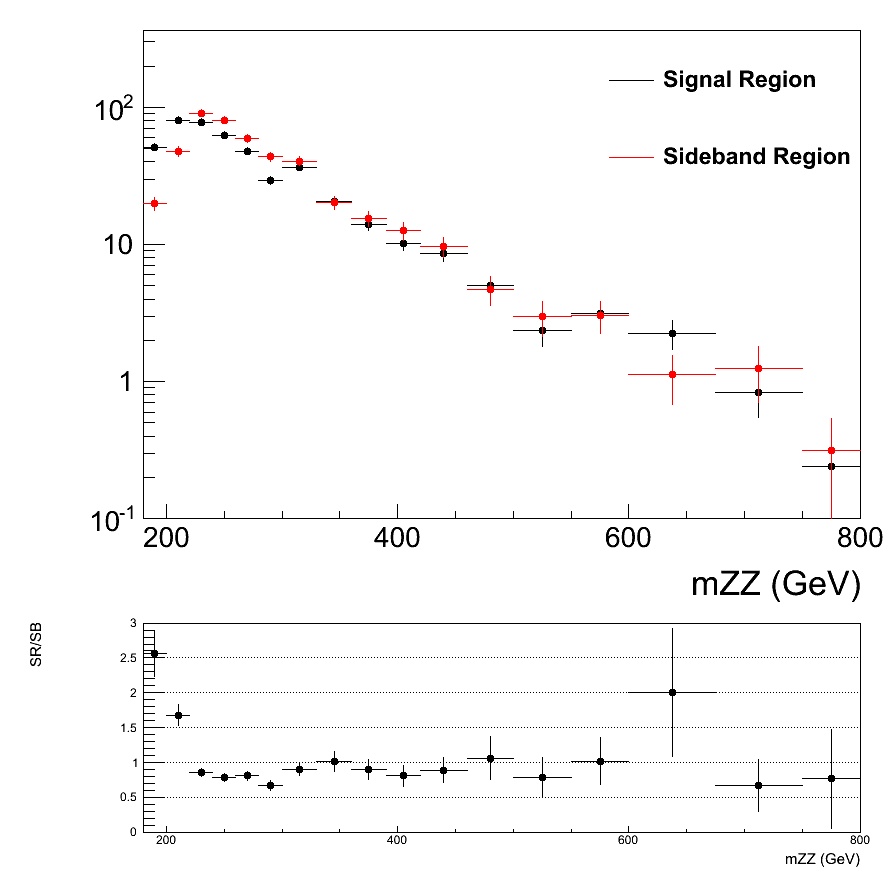
\includegraphics[width=0.33\textwidth]{plots/approvalxchecks/mZZ_SRvsSB_lep1_2btags_Log.png}
}
\caption{Mass distributions of the $\LL jj$ system for events in the simualted sideband and signal regions for the elctron (left)
 and muon (right) channels. From top to bottom, plots
correspond to the 0-, 1-, and 2-btag categories. 
\label{fig:clos}
}
\end{figure}


\subsection{}
Figure~\ref{fig:lrline} to~\ref{fig:lrlogmu} show the sideband data compared to the background prediction separately for the left and right sideband. While the background shapes are noticeably different between the left and right sideband, both agree well between data nad simulation, giving conifdence that the description is similarly good in the signal region. 


\begin{figure}[htb]
\centerline{
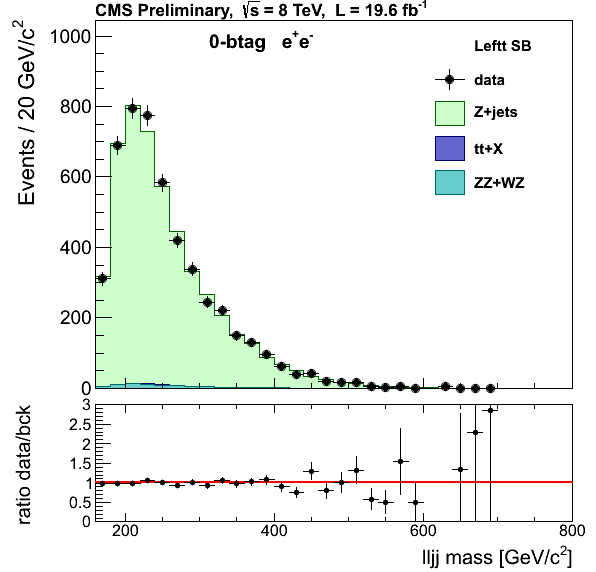
\includegraphics[width=0.33\textwidth]{plots/approvalxchecks/Left_0b_eelin.png}
\includegraphics[width=0.33\textwidth]{plots/approvalxchecks/Right_0b_eelin.png}
}
\centerline{
\includegraphics[width=0.33\textwidth]{plots/approvalxchecks/Left_1b_eelin.png}
\includegraphics[width=0.33\textwidth]{plots/approvalxchecks/Right_1b_eelin.png}
}
\centerline{
\includegraphics[width=0.33\textwidth]{plots/approvalxchecks/Left_2b_eelin.png}
\includegraphics[width=0.33\textwidth]{plots/approvalxchecks/Right_2b_eelin.png}
}
\caption{Mass distributions of the $\LL jj$ system for events in the left (left)
 and right (right) sideband regions in the electron channel. From top to bottom, plots
correspond to the 0-, 1-, and 2-btag categories. 
The dots are data, pale green histogram corrected Z+jets simulation,
light blue simulated diboson background and dark blue $\ttbar$ events from data (which
include single top, WW, $\Zo\to\TT$+jets).
\label{fig:lrline}
}
\end{figure}

\begin{figure}[htb]
\centerline{
\includegraphics[width=0.33\textwidth]{plots/approvalxchecks/Left_0b_mmlin.png}
\includegraphics[width=0.33\textwidth]{plots/approvalxchecks/Right_0b_mmlin.png}
}
\centerline{
\includegraphics[width=0.33\textwidth]{plots/approvalxchecks/Left_1b_mmlin.png}
\includegraphics[width=0.33\textwidth]{plots/approvalxchecks/Right_1b_mmlin.png}
}
\centerline{
\includegraphics[width=0.33\textwidth]{plots/approvalxchecks/Left_2b_mmlin.png}
\includegraphics[width=0.33\textwidth]{plots/approvalxchecks/Right_2b_mmlin.png}
}
\caption{Same Figure~\ref{fig:lrline} but in themuon channel.
\label{fig:lrlinmu}
}
\end{figure}

\begin{figure}[htb]
\centerline{
\includegraphics[width=0.33\textwidth]{plots/approvalxchecks/Left_0b_ee.png}
\includegraphics[width=0.33\textwidth]{plots/approvalxchecks/Right_0b_ee.png}
}
\centerline{
\includegraphics[width=0.33\textwidth]{plots/approvalxchecks/Left_1b_ee.png}
\includegraphics[width=0.33\textwidth]{plots/approvalxchecks/Right_1b_ee.png}
}
\centerline{
\includegraphics[width=0.33\textwidth]{plots/approvalxchecks/Left_2b_ee.png}
\includegraphics[width=0.33\textwidth]{plots/approvalxchecks/Right_2b_ee.png}
}
\caption{Same Figure~\ref{fig:lrline} but in themuon channellogarithmic scale.
\label{fig:lrloge}
}
\end{figure}

\begin{figure}[htb]
\centerline{
\includegraphics[width=0.33\textwidth]{plots/approvalxchecks/Left_0b_mm.png}
\includegraphics[width=0.33\textwidth]{plots/approvalxchecks/Right_0b_mm.png}
}
\centerline{
\includegraphics[width=0.33\textwidth]{plots/approvalxchecks/Left_1b_mm.png}
\includegraphics[width=0.33\textwidth]{plots/approvalxchecks/Right_1b_mm.png}
}
\centerline{
\includegraphics[width=0.33\textwidth]{plots/approvalxchecks/Left_2b_mm.png}
\includegraphics[width=0.33\textwidth]{plots/approvalxchecks/Right_2b_mm.png}
}
\caption{Same Figure~\ref{fig:lrlinmu} but in themuon channellogarithmic scale.
\label{fig:lrlogmu}
}
\end{figure}


\subsection{}
We have three independent analyses (different codes, ntuples, etc.) which agree 
well at the sub-percent level, in the numbers of events and shapes of the 
distributions. We have also checked the final limits, calculated both with the 
official combine tool and with an independent home-made code, and give 
consistent results. These checks have been reported in HZZ meetings and at the 
pre-approval session.

We are confident that no bug is present that gives visible effects.

\subsection{}
see section~\ref{sec:results}

\subsection{}
This has been addressed in the PAS. For internal documentation we keep the wider range in this note.




